% Options for packages loaded elsewhere
\PassOptionsToPackage{unicode}{hyperref}
\PassOptionsToPackage{hyphens}{url}
%
\documentclass[
]{article}
\usepackage{amsmath,amssymb}
\usepackage{lmodern}
\usepackage{ifxetex,ifluatex}
\ifnum 0\ifxetex 1\fi\ifluatex 1\fi=0 % if pdftex
  \usepackage[T1]{fontenc}
  \usepackage[utf8]{inputenc}
  \usepackage{textcomp} % provide euro and other symbols
\else % if luatex or xetex
  \usepackage{unicode-math}
  \defaultfontfeatures{Scale=MatchLowercase}
  \defaultfontfeatures[\rmfamily]{Ligatures=TeX,Scale=1}
\fi
% Use upquote if available, for straight quotes in verbatim environments
\IfFileExists{upquote.sty}{\usepackage{upquote}}{}
\IfFileExists{microtype.sty}{% use microtype if available
  \usepackage[]{microtype}
  \UseMicrotypeSet[protrusion]{basicmath} % disable protrusion for tt fonts
}{}
\makeatletter
\@ifundefined{KOMAClassName}{% if non-KOMA class
  \IfFileExists{parskip.sty}{%
    \usepackage{parskip}
  }{% else
    \setlength{\parindent}{0pt}
    \setlength{\parskip}{6pt plus 2pt minus 1pt}}
}{% if KOMA class
  \KOMAoptions{parskip=half}}
\makeatother
\usepackage{xcolor}
\IfFileExists{xurl.sty}{\usepackage{xurl}}{} % add URL line breaks if available
\IfFileExists{bookmark.sty}{\usepackage{bookmark}}{\usepackage{hyperref}}
\hypersetup{
  pdftitle={Semester Project Exploratory Data Analysis},
  pdfauthor={Logan Herrmeyer},
  hidelinks,
  pdfcreator={LaTeX via pandoc}}
\urlstyle{same} % disable monospaced font for URLs
\usepackage[margin=1in]{geometry}
\usepackage{color}
\usepackage{fancyvrb}
\newcommand{\VerbBar}{|}
\newcommand{\VERB}{\Verb[commandchars=\\\{\}]}
\DefineVerbatimEnvironment{Highlighting}{Verbatim}{commandchars=\\\{\}}
% Add ',fontsize=\small' for more characters per line
\usepackage{framed}
\definecolor{shadecolor}{RGB}{248,248,248}
\newenvironment{Shaded}{\begin{snugshade}}{\end{snugshade}}
\newcommand{\AlertTok}[1]{\textcolor[rgb]{0.94,0.16,0.16}{#1}}
\newcommand{\AnnotationTok}[1]{\textcolor[rgb]{0.56,0.35,0.01}{\textbf{\textit{#1}}}}
\newcommand{\AttributeTok}[1]{\textcolor[rgb]{0.77,0.63,0.00}{#1}}
\newcommand{\BaseNTok}[1]{\textcolor[rgb]{0.00,0.00,0.81}{#1}}
\newcommand{\BuiltInTok}[1]{#1}
\newcommand{\CharTok}[1]{\textcolor[rgb]{0.31,0.60,0.02}{#1}}
\newcommand{\CommentTok}[1]{\textcolor[rgb]{0.56,0.35,0.01}{\textit{#1}}}
\newcommand{\CommentVarTok}[1]{\textcolor[rgb]{0.56,0.35,0.01}{\textbf{\textit{#1}}}}
\newcommand{\ConstantTok}[1]{\textcolor[rgb]{0.00,0.00,0.00}{#1}}
\newcommand{\ControlFlowTok}[1]{\textcolor[rgb]{0.13,0.29,0.53}{\textbf{#1}}}
\newcommand{\DataTypeTok}[1]{\textcolor[rgb]{0.13,0.29,0.53}{#1}}
\newcommand{\DecValTok}[1]{\textcolor[rgb]{0.00,0.00,0.81}{#1}}
\newcommand{\DocumentationTok}[1]{\textcolor[rgb]{0.56,0.35,0.01}{\textbf{\textit{#1}}}}
\newcommand{\ErrorTok}[1]{\textcolor[rgb]{0.64,0.00,0.00}{\textbf{#1}}}
\newcommand{\ExtensionTok}[1]{#1}
\newcommand{\FloatTok}[1]{\textcolor[rgb]{0.00,0.00,0.81}{#1}}
\newcommand{\FunctionTok}[1]{\textcolor[rgb]{0.00,0.00,0.00}{#1}}
\newcommand{\ImportTok}[1]{#1}
\newcommand{\InformationTok}[1]{\textcolor[rgb]{0.56,0.35,0.01}{\textbf{\textit{#1}}}}
\newcommand{\KeywordTok}[1]{\textcolor[rgb]{0.13,0.29,0.53}{\textbf{#1}}}
\newcommand{\NormalTok}[1]{#1}
\newcommand{\OperatorTok}[1]{\textcolor[rgb]{0.81,0.36,0.00}{\textbf{#1}}}
\newcommand{\OtherTok}[1]{\textcolor[rgb]{0.56,0.35,0.01}{#1}}
\newcommand{\PreprocessorTok}[1]{\textcolor[rgb]{0.56,0.35,0.01}{\textit{#1}}}
\newcommand{\RegionMarkerTok}[1]{#1}
\newcommand{\SpecialCharTok}[1]{\textcolor[rgb]{0.00,0.00,0.00}{#1}}
\newcommand{\SpecialStringTok}[1]{\textcolor[rgb]{0.31,0.60,0.02}{#1}}
\newcommand{\StringTok}[1]{\textcolor[rgb]{0.31,0.60,0.02}{#1}}
\newcommand{\VariableTok}[1]{\textcolor[rgb]{0.00,0.00,0.00}{#1}}
\newcommand{\VerbatimStringTok}[1]{\textcolor[rgb]{0.31,0.60,0.02}{#1}}
\newcommand{\WarningTok}[1]{\textcolor[rgb]{0.56,0.35,0.01}{\textbf{\textit{#1}}}}
\usepackage{longtable,booktabs,array}
\usepackage{calc} % for calculating minipage widths
% Correct order of tables after \paragraph or \subparagraph
\usepackage{etoolbox}
\makeatletter
\patchcmd\longtable{\par}{\if@noskipsec\mbox{}\fi\par}{}{}
\makeatother
% Allow footnotes in longtable head/foot
\IfFileExists{footnotehyper.sty}{\usepackage{footnotehyper}}{\usepackage{footnote}}
\makesavenoteenv{longtable}
\usepackage{graphicx}
\makeatletter
\def\maxwidth{\ifdim\Gin@nat@width>\linewidth\linewidth\else\Gin@nat@width\fi}
\def\maxheight{\ifdim\Gin@nat@height>\textheight\textheight\else\Gin@nat@height\fi}
\makeatother
% Scale images if necessary, so that they will not overflow the page
% margins by default, and it is still possible to overwrite the defaults
% using explicit options in \includegraphics[width, height, ...]{}
\setkeys{Gin}{width=\maxwidth,height=\maxheight,keepaspectratio}
% Set default figure placement to htbp
\makeatletter
\def\fps@figure{htbp}
\makeatother
\setlength{\emergencystretch}{3em} % prevent overfull lines
\providecommand{\tightlist}{%
  \setlength{\itemsep}{0pt}\setlength{\parskip}{0pt}}
\setcounter{secnumdepth}{-\maxdimen} % remove section numbering
\ifluatex
  \usepackage{selnolig}  % disable illegal ligatures
\fi

\title{Semester Project Exploratory Data Analysis}
\author{Logan Herrmeyer}
\date{June 22, 2021}

\begin{document}
\maketitle

{
\setcounter{tocdepth}{2}
\tableofcontents
}
\begin{Shaded}
\begin{Highlighting}[]
\FunctionTok{library}\NormalTok{(pacman)}
\CommentTok{\#devtools::install\_github("deleetdk/USA.county.data")}
\NormalTok{pacman}\SpecialCharTok{::}\FunctionTok{p\_load}\NormalTok{(tidyverse, maps, tree, USA.county.data)}
\NormalTok{pacman}\SpecialCharTok{::}\FunctionTok{p\_load}\NormalTok{(rpart, rpart.plot, rattle, readxl)}
\CommentTok{\#data(USA\_county\_data)}
\CommentTok{\#d \textless{}{-} read\_csv("https://github.com/Deleetdk/USA.county.data/blob/master/Scrape\%20and\%20tidy\%20code/data/tidy\_data.csv?raw=true")}
\FunctionTok{data}\NormalTok{(USA\_county\_data)}
\NormalTok{d }\OtherTok{\textless{}{-}}\NormalTok{ USA\_county\_data}
\CommentTok{\# Remove leftover statistical data and bad weather data}
\CommentTok{\# https://openpsych.net/paper/12/}
\NormalTok{ex\_cols }\OtherTok{=} \FunctionTok{c}\NormalTok{(}\StringTok{"S"}\NormalTok{,}\StringTok{"CA"}\NormalTok{,}\StringTok{"MAR"}\NormalTok{,}\StringTok{"CFS"}\NormalTok{,}\StringTok{"ACFS"}\NormalTok{,}\StringTok{"MeanALC"}\NormalTok{,}\StringTok{"MaxALC"}\NormalTok{,}\StringTok{"X"}\NormalTok{,}\StringTok{"Y"}\NormalTok{)}
\NormalTok{d }\OtherTok{\textless{}{-}}\NormalTok{ d }\SpecialCharTok{\%\textgreater{}\%}
  \FunctionTok{select}\NormalTok{(}\SpecialCharTok{{-}}\FunctionTok{one\_of}\NormalTok{(ex\_cols)) }\SpecialCharTok{\%\textgreater{}\%}
  \FunctionTok{select}\NormalTok{(}\SpecialCharTok{!}\FunctionTok{matches}\NormalTok{(}\StringTok{"\_(PRCP|TMAX|TMIN|TAVG)"}\NormalTok{)) }\SpecialCharTok{\%\textgreater{}\%}
  \FunctionTok{select}\NormalTok{(}\SpecialCharTok{!}\FunctionTok{matches}\NormalTok{(}\StringTok{"\_bins"}\NormalTok{))}
\NormalTok{d }\OtherTok{\textless{}{-}}\NormalTok{ d }\SpecialCharTok{\%\textgreater{}\%}
  \FunctionTok{mutate}\NormalTok{(}\AttributeTok{prec\_pop =}\NormalTok{ Total.Population}\SpecialCharTok{/}\NormalTok{precincts)}

\CommentTok{\# Get area/pop dens data}
\NormalTok{area }\OtherTok{\textless{}{-}} \FunctionTok{read\_excel}\NormalTok{(}\StringTok{"land\_area.xls"}\NormalTok{)}
\NormalTok{county\_area }\OtherTok{\textless{}{-}}\NormalTok{ area }\SpecialCharTok{\%\textgreater{}\%}
    \FunctionTok{rename}\NormalTok{(}\AttributeTok{land\_area=}\NormalTok{LND010200D) }\SpecialCharTok{\%\textgreater{}\%}
    \FunctionTok{mutate}\NormalTok{(}\AttributeTok{fips=}\FunctionTok{as.numeric}\NormalTok{(STCOU)) }\SpecialCharTok{\%\textgreater{}\%}
    \FunctionTok{select}\NormalTok{(fips,land\_area)}
\NormalTok{d }\OtherTok{\textless{}{-}} \FunctionTok{inner\_join}\NormalTok{(d, county\_area, }\AttributeTok{by=}\StringTok{"fips"}\NormalTok{)}
\NormalTok{d }\OtherTok{\textless{}{-}}\NormalTok{ d }\SpecialCharTok{\%\textgreater{}\%}
  \FunctionTok{mutate}\NormalTok{(}\AttributeTok{pop\_dens =}\NormalTok{ Total.Population}\SpecialCharTok{/}\NormalTok{land\_area) }\SpecialCharTok{\%\textgreater{}\%}
  \FunctionTok{mutate}\NormalTok{(}\AttributeTok{log\_pd =} \FunctionTok{log}\NormalTok{(pop\_dens)) }\SpecialCharTok{\%\textgreater{}\%}
  \FunctionTok{mutate}\NormalTok{(}\AttributeTok{log\_pop =} \FunctionTok{log}\NormalTok{(Total.Population)) }\SpecialCharTok{\%\textgreater{}\%}
  \FunctionTok{mutate}\NormalTok{(}\AttributeTok{log\_pc =} \FunctionTok{log}\NormalTok{(precincts)) }\SpecialCharTok{\%\textgreater{}\%}
  \FunctionTok{mutate}\NormalTok{(}\AttributeTok{ppc =}\NormalTok{ precincts}\SpecialCharTok{/}\NormalTok{Total.Population) }\SpecialCharTok{\%\textgreater{}\%}
  \FunctionTok{filter}\NormalTok{(land\_area }\SpecialCharTok{\textgreater{}} \DecValTok{0}\NormalTok{) }\SpecialCharTok{\%\textgreater{}\%}
  \FunctionTok{filter}\NormalTok{(}\SpecialCharTok{!}\FunctionTok{is.na}\NormalTok{(pop\_dens)) }\SpecialCharTok{\%\textgreater{}\%}
  \FunctionTok{filter}\NormalTok{(}\SpecialCharTok{!}\FunctionTok{is.infinite}\NormalTok{(pop\_dens))}
\end{Highlighting}
\end{Shaded}

\hypertarget{correlations}{%
\subsection{Correlations}\label{correlations}}

\hypertarget{for-all-variables}{%
\subsubsection{For all variables}\label{for-all-variables}}

\begin{Shaded}
\begin{Highlighting}[]
\NormalTok{d\_numeric }\OtherTok{\textless{}{-}}\NormalTok{ d[, }\FunctionTok{unlist}\NormalTok{(}\FunctionTok{lapply}\NormalTok{(d, is.numeric))]}
\NormalTok{correlations }\OtherTok{\textless{}{-}} \FunctionTok{as.data.frame}\NormalTok{(}\FunctionTok{cor}\NormalTok{(}
\NormalTok{  d\_numeric, }\AttributeTok{use=}\StringTok{"pairwise.complete.obs"}
\NormalTok{))}
\end{Highlighting}
\end{Shaded}

\begin{verbatim}
## Warning in cor(d_numeric, use = "pairwise.complete.obs"): the standard deviation
## is zero
\end{verbatim}

\begin{Shaded}
\begin{Highlighting}[]
\NormalTok{cor\_df\_1 }\OtherTok{\textless{}{-}}\NormalTok{ correlations }\SpecialCharTok{\%\textgreater{}\%} 
  \FunctionTok{select}\NormalTok{(rep16\_frac) }\SpecialCharTok{\%\textgreater{}\%}
  \FunctionTok{arrange}\NormalTok{(}\SpecialCharTok{{-}}\FunctionTok{abs}\NormalTok{(rep16\_frac))}
\NormalTok{knitr}\SpecialCharTok{::}\FunctionTok{kable}\NormalTok{(cor\_df\_1 }\SpecialCharTok{\%\textgreater{}\%} \FunctionTok{head}\NormalTok{(}\DecValTok{15}\NormalTok{))}
\end{Highlighting}
\end{Shaded}

\begin{longtable}[]{@{}lr@{}}
\toprule
& rep16\_frac \\
\midrule
\endhead
rep16\_frac & 1.0000000 \\
rep16\_frac2 & 0.9918778 \\
dem16\_frac2 & -0.9918778 \\
dem16\_frac & -0.9834403 \\
rep12\_frac2 & 0.9354249 \\
dem12\_frac2 & -0.9354249 \\
dem12\_frac & -0.9348959 \\
rep12\_frac & 0.9345204 \\
dem08\_frac & -0.9084699 \\
rep08\_frac2 & 0.9056343 \\
dem08\_frac2 & -0.9056343 \\
rep08\_frac & 0.9019726 \\
votes16\_duncanr & -0.7862420 \\
votes16\_none\_of\_these\_candidates & -0.7278439 \\
votes16\_giordanir & -0.5379842 \\
\bottomrule
\end{longtable}

\hypertarget{not-counting-previous-voting}{%
\subsubsection{Not counting previous
voting}\label{not-counting-previous-voting}}

\begin{Shaded}
\begin{Highlighting}[]
\NormalTok{d\_numeric }\OtherTok{\textless{}{-}}\NormalTok{ d[, }\FunctionTok{unlist}\NormalTok{(}\FunctionTok{lapply}\NormalTok{(d, is.numeric))]}
\NormalTok{d\_cor }\OtherTok{\textless{}{-}}\NormalTok{ d\_numeric }\SpecialCharTok{\%\textgreater{}\%} 
    \FunctionTok{select}\NormalTok{(}\SpecialCharTok{!}\FunctionTok{starts\_with}\NormalTok{(}\StringTok{"vote"}\NormalTok{)) }\SpecialCharTok{\%\textgreater{}\%}
    \FunctionTok{select}\NormalTok{(}\SpecialCharTok{!}\FunctionTok{matches}\NormalTok{(}\StringTok{"...(08|12)\_frac.*"}\NormalTok{)) }\SpecialCharTok{\%\textgreater{}\%}
    \FunctionTok{select}\NormalTok{(}\SpecialCharTok{!}\FunctionTok{matches}\NormalTok{(}\StringTok{"[a{-}z][0{-}9][0{-}9]$"}\NormalTok{)) }\SpecialCharTok{\%\textgreater{}\%}
    \FunctionTok{select}\NormalTok{(}\SpecialCharTok{!}\FunctionTok{ends\_with}\NormalTok{(}\StringTok{"frac2"}\NormalTok{))}
\NormalTok{d\_cor }\OtherTok{\textless{}{-}} 
\NormalTok{  d\_cor[,}\SpecialCharTok{!}\FunctionTok{grepl}\NormalTok{(}\StringTok{"(?\textless{}!rep)16\_frac.*"}\NormalTok{,}\FunctionTok{colnames}\NormalTok{(d\_cor),}\AttributeTok{perl=}\NormalTok{T)]}

\NormalTok{correlations\_2 }\OtherTok{\textless{}{-}} \FunctionTok{as.data.frame}\NormalTok{(}\FunctionTok{cor}\NormalTok{(}
\NormalTok{  d\_cor, }\AttributeTok{use=}\StringTok{"pairwise.complete.obs"}\NormalTok{, }\AttributeTok{method=}\StringTok{"pearson"}
\NormalTok{))}

\NormalTok{cor\_df\_2 }\OtherTok{\textless{}{-}}\NormalTok{ correlations\_2 }\SpecialCharTok{\%\textgreater{}\%} 
  \FunctionTok{select}\NormalTok{(rep16\_frac) }\SpecialCharTok{\%\textgreater{}\%}
  \FunctionTok{arrange}\NormalTok{(}\SpecialCharTok{{-}}\FunctionTok{abs}\NormalTok{(rep16\_frac)) }\SpecialCharTok{\%\textgreater{}\%}
  \FunctionTok{distinct}\NormalTok{(rep16\_frac, }\AttributeTok{.keep\_all =}\NormalTok{ T)}
\NormalTok{knitr}\SpecialCharTok{::}\FunctionTok{kable}\NormalTok{(cor\_df\_2 }\SpecialCharTok{\%\textgreater{}\%} \FunctionTok{head}\NormalTok{(}\DecValTok{15}\NormalTok{))}
\end{Highlighting}
\end{Shaded}

\begin{longtable}[]{@{}lr@{}}
\toprule
& rep16\_frac \\
\midrule
\endhead
rep16\_frac & 1.0000000 \\
White.not.Latino.Population & 0.5378038 \\
Graduate.Degree & -0.5342947 \\
log\_pop & -0.5071902 \\
White\_Asian & 0.4986800 \\
At.Least.Bachelor.s.Degree & -0.4930385 \\
Sexually.transmitted.infections & -0.4754802 \\
log\_pd & -0.4604581 \\
log\_pc & -0.4531320 \\
Asian.American.Population & -0.4348100 \\
SIRE\_homogeneity & 0.4155649 \\
African.American.Population & -0.4150909 \\
HIV.prevalence.rate & -0.4001711 \\
Mixedness & -0.3886669 \\
Children.in.single.parent.households & -0.3813384 \\
\bottomrule
\end{longtable}

\hypertarget{using-spearman-method}{%
\subsubsection{Using Spearman method}\label{using-spearman-method}}

\begin{Shaded}
\begin{Highlighting}[]
\NormalTok{d\_numeric }\OtherTok{\textless{}{-}}\NormalTok{ d[, }\FunctionTok{unlist}\NormalTok{(}\FunctionTok{lapply}\NormalTok{(d, is.numeric))]}
\NormalTok{d\_cor }\OtherTok{\textless{}{-}}\NormalTok{ d\_numeric }\SpecialCharTok{\%\textgreater{}\%} 
    \FunctionTok{select}\NormalTok{(}\SpecialCharTok{!}\FunctionTok{starts\_with}\NormalTok{(}\StringTok{"vote"}\NormalTok{)) }\SpecialCharTok{\%\textgreater{}\%}
    \FunctionTok{select}\NormalTok{(}\SpecialCharTok{!}\FunctionTok{matches}\NormalTok{(}\StringTok{"...(08|12)\_frac.*"}\NormalTok{)) }\SpecialCharTok{\%\textgreater{}\%}
    \FunctionTok{select}\NormalTok{(}\SpecialCharTok{!}\FunctionTok{matches}\NormalTok{(}\StringTok{"[a{-}z][0{-}9][0{-}9]$"}\NormalTok{)) }\SpecialCharTok{\%\textgreater{}\%}
    \FunctionTok{select}\NormalTok{(}\SpecialCharTok{!}\FunctionTok{ends\_with}\NormalTok{(}\StringTok{"frac2"}\NormalTok{))}
\NormalTok{d\_cor }\OtherTok{\textless{}{-}} 
\NormalTok{  d\_cor[,}\SpecialCharTok{!}\FunctionTok{grepl}\NormalTok{(}\StringTok{"(?\textless{}!rep)16\_frac.*"}\NormalTok{,}\FunctionTok{colnames}\NormalTok{(d\_cor),}\AttributeTok{perl=}\NormalTok{T)]}

\NormalTok{correlations\_3 }\OtherTok{\textless{}{-}} \FunctionTok{as.data.frame}\NormalTok{(}\FunctionTok{cor}\NormalTok{(}
\NormalTok{  d\_cor, }\AttributeTok{use=}\StringTok{"pairwise.complete.obs"}\NormalTok{, }\AttributeTok{method=}\StringTok{"spearman"}
\NormalTok{))}

\NormalTok{cor\_df\_3 }\OtherTok{\textless{}{-}}\NormalTok{ correlations\_3 }\SpecialCharTok{\%\textgreater{}\%} 
  \FunctionTok{select}\NormalTok{(rep16\_frac) }\SpecialCharTok{\%\textgreater{}\%}
  \FunctionTok{arrange}\NormalTok{(}\SpecialCharTok{{-}}\FunctionTok{abs}\NormalTok{(rep16\_frac)) }\SpecialCharTok{\%\textgreater{}\%}
  \FunctionTok{distinct}\NormalTok{(rep16\_frac, }\AttributeTok{.keep\_all =}\NormalTok{ T)}
\NormalTok{knitr}\SpecialCharTok{::}\FunctionTok{kable}\NormalTok{(cor\_df\_3 }\SpecialCharTok{\%\textgreater{}\%} \FunctionTok{head}\NormalTok{(}\DecValTok{15}\NormalTok{))}
\end{Highlighting}
\end{Shaded}

\begin{longtable}[]{@{}lr@{}}
\toprule
& rep16\_frac \\
\midrule
\endhead
rep16\_frac & 1.0000000 \\
Asian.American.Population & -0.5002842 \\
Total.Population & -0.4766693 \\
Graduate.Degree & -0.4578545 \\
White.not.Latino.Population & 0.4360950 \\
precincts & -0.4205529 \\
reporting & -0.4191627 \\
Injury.deaths & 0.4157215 \\
At.Least.Bachelor.s.Degree & -0.4139711 \\
Sexually.transmitted.infections & -0.4110872 \\
pop\_dens & -0.4069272 \\
White\_Asian & 0.4015622 \\
SIRE\_homogeneity & 0.4008215 \\
Construction.extraction.maintenance.and.repair.occupations &
0.3879461 \\
HIV.prevalence.rate & -0.3804431 \\
\bottomrule
\end{longtable}

\hypertarget{linear-correlation-graphs}{%
\subsection{Linear correlation graphs}\label{linear-correlation-graphs}}

\begin{Shaded}
\begin{Highlighting}[]
\NormalTok{lin\_vars }\OtherTok{\textless{}{-}} \FunctionTok{rownames}\NormalTok{(cor\_df\_2 }\SpecialCharTok{\%\textgreater{}\%} \FunctionTok{head}\NormalTok{(}\DecValTok{8}\NormalTok{))}
\ControlFlowTok{for}\NormalTok{(var }\ControlFlowTok{in}\NormalTok{ lin\_vars)\{}
\NormalTok{  plot }\OtherTok{\textless{}{-}} \FunctionTok{ggplot}\NormalTok{(}\FunctionTok{aes\_string}\NormalTok{(}\AttributeTok{x=}\NormalTok{var,}\AttributeTok{y=}\StringTok{"rep16\_frac"}\NormalTok{),}\AttributeTok{data=}\NormalTok{d) }\SpecialCharTok{+}
    \FunctionTok{geom\_point}\NormalTok{() }\SpecialCharTok{+}
    \FunctionTok{geom\_smooth}\NormalTok{(}\AttributeTok{method=}\StringTok{"lm"}\NormalTok{) }\SpecialCharTok{+}
    \FunctionTok{theme\_bw}\NormalTok{() }\SpecialCharTok{+}
    \FunctionTok{labs}\NormalTok{(}
      \AttributeTok{title =} \FunctionTok{paste}\NormalTok{(}\StringTok{"Republican fraction in 2016 vs"}\NormalTok{,var,}
                    \StringTok{" r="}\NormalTok{,}\FunctionTok{round}\NormalTok{(cor\_df\_2[var,],}\DecValTok{3}\NormalTok{))}
\NormalTok{    )}
  \FunctionTok{print}\NormalTok{(plot)}
\NormalTok{\}}
\end{Highlighting}
\end{Shaded}

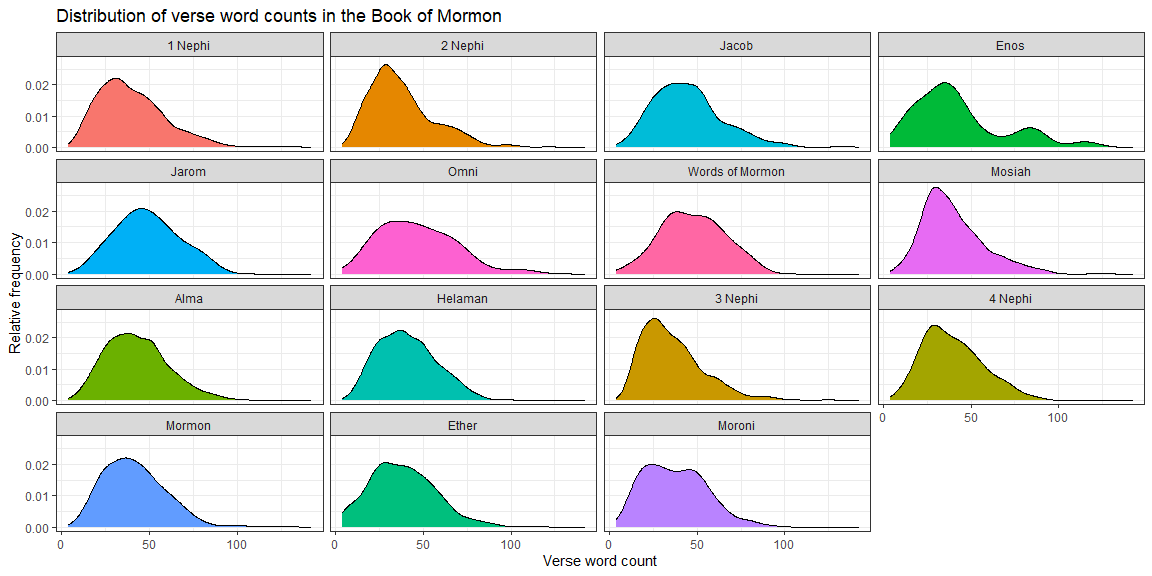
\includegraphics{eda_files/figure-latex/unnamed-chunk-6-1.pdf}
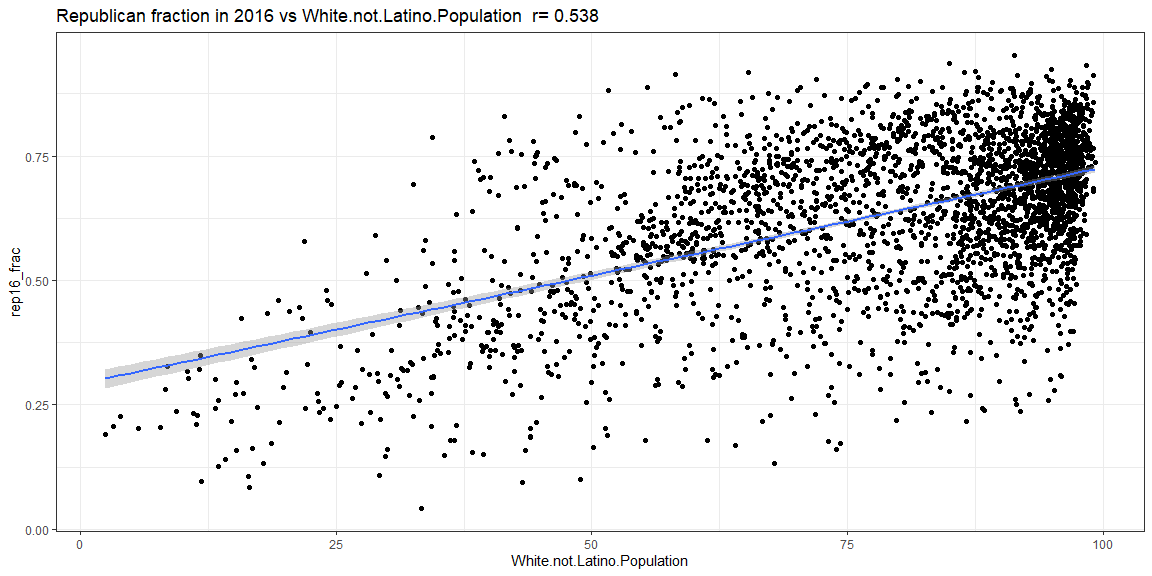
\includegraphics{eda_files/figure-latex/unnamed-chunk-6-2.pdf}
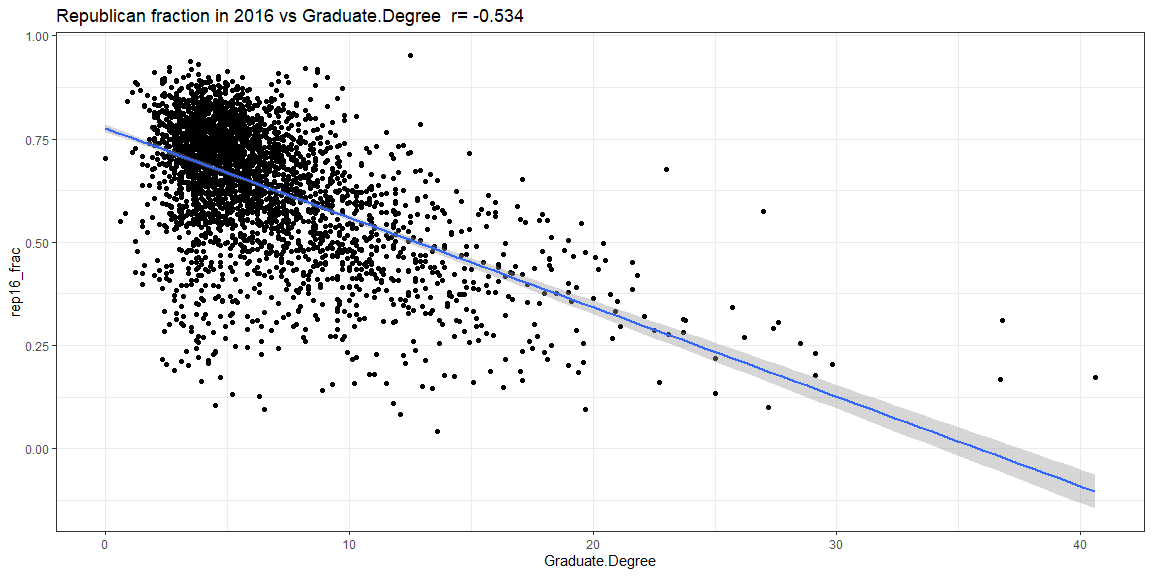
\includegraphics{eda_files/figure-latex/unnamed-chunk-6-3.pdf}
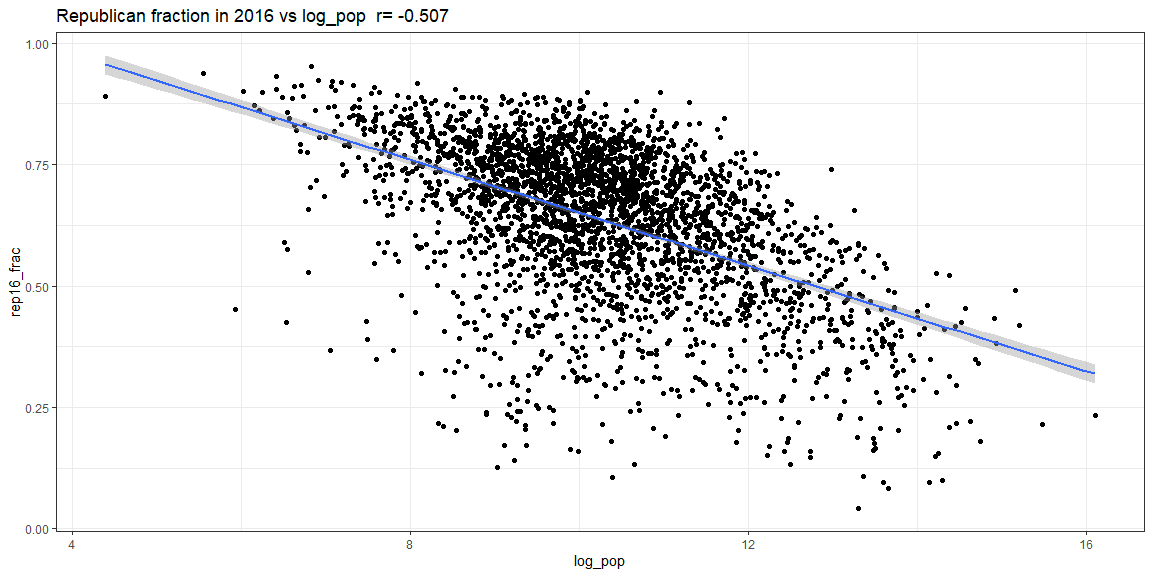
\includegraphics{eda_files/figure-latex/unnamed-chunk-6-4.pdf}
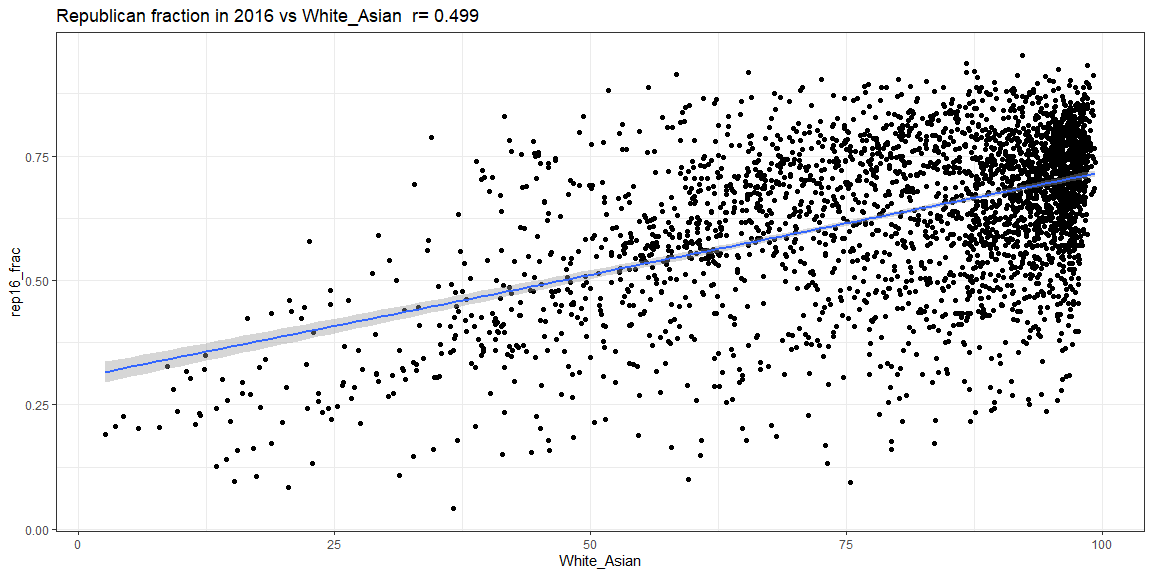
\includegraphics{eda_files/figure-latex/unnamed-chunk-6-5.pdf}
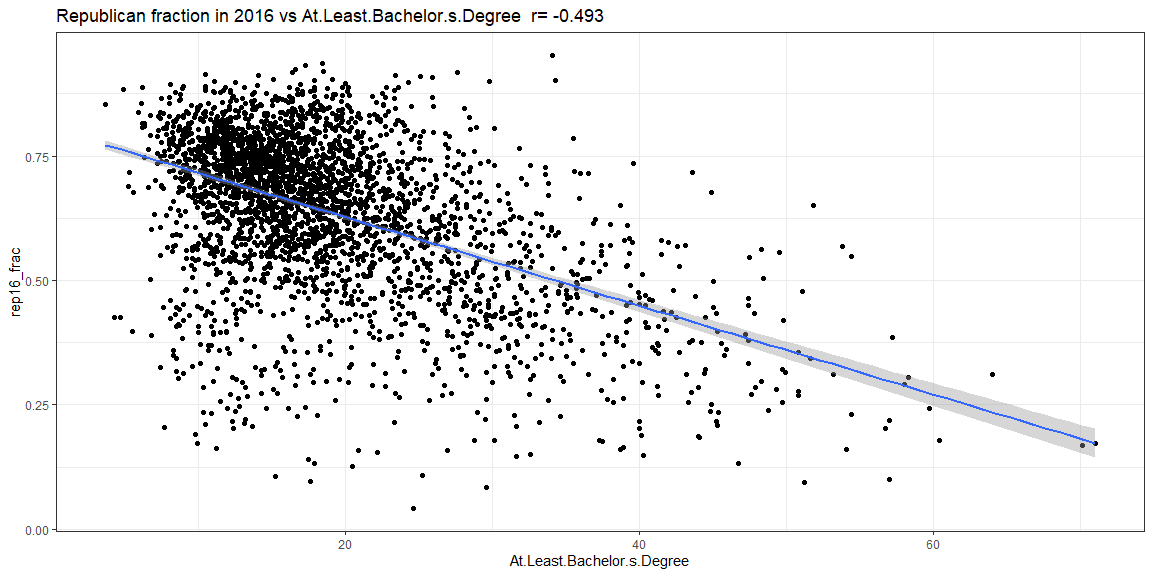
\includegraphics{eda_files/figure-latex/unnamed-chunk-6-6.pdf}
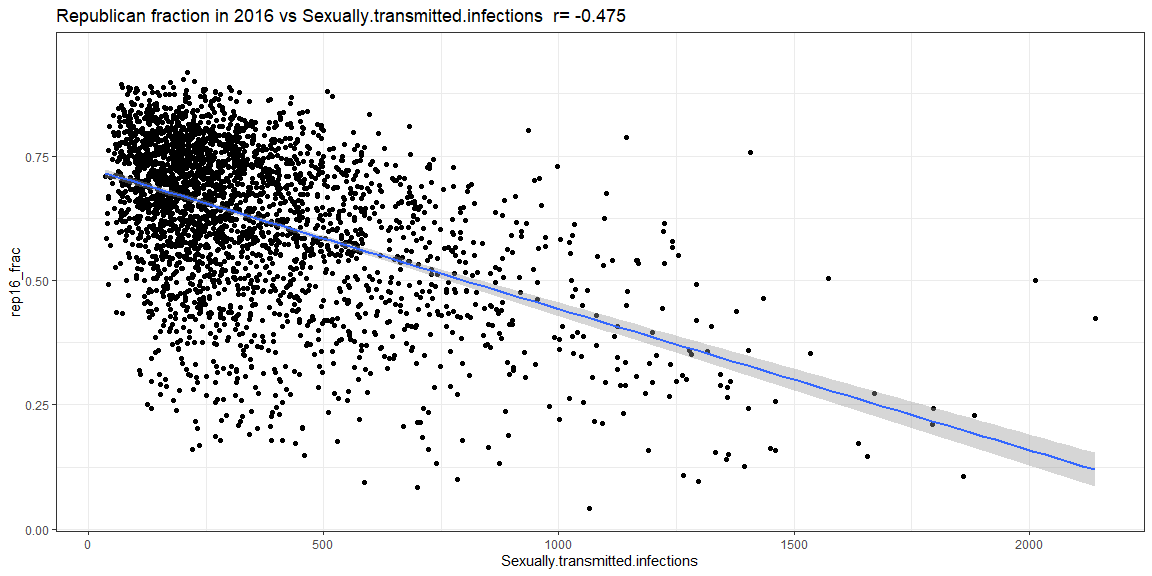
\includegraphics{eda_files/figure-latex/unnamed-chunk-6-7.pdf}
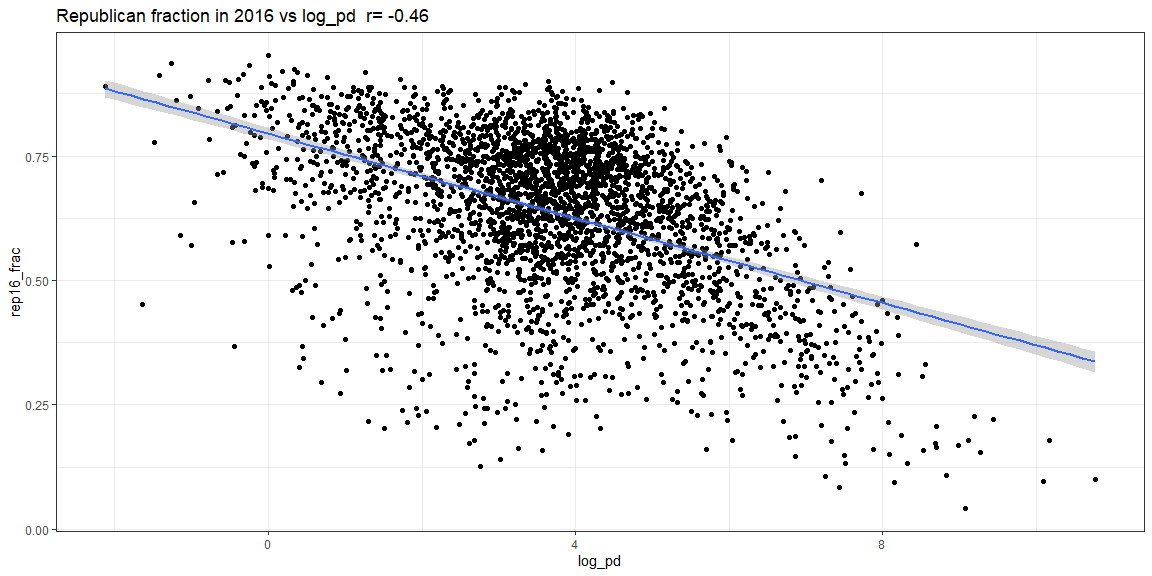
\includegraphics{eda_files/figure-latex/unnamed-chunk-6-8.pdf}

\hypertarget{other-monotonic-correlations}{%
\subsection{Other monotonic
correlations}\label{other-monotonic-correlations}}

\begin{Shaded}
\begin{Highlighting}[]
\NormalTok{cor\_m\_df }\OtherTok{\textless{}{-}} \FunctionTok{inner\_join}\NormalTok{(}
\NormalTok{  (cor\_df\_3 }\SpecialCharTok{\%\textgreater{}\%} \FunctionTok{mutate}\NormalTok{(}\AttributeTok{nam =} \FunctionTok{rownames}\NormalTok{(cor\_df\_3))),}
\NormalTok{  (cor\_df\_2 }\SpecialCharTok{\%\textgreater{}\%} \FunctionTok{mutate}\NormalTok{(}\AttributeTok{nam =} \FunctionTok{rownames}\NormalTok{(cor\_df\_2))),}
  \AttributeTok{by=}\StringTok{"nam"}
\NormalTok{) }\SpecialCharTok{\%\textgreater{}\%} \FunctionTok{filter}\NormalTok{(}\FunctionTok{abs}\NormalTok{(rep16\_frac.x) }\SpecialCharTok{\textgreater{}} \FunctionTok{abs}\NormalTok{(rep16\_frac.y))}
\NormalTok{m\_vars }\OtherTok{\textless{}{-}}\NormalTok{ cor\_m\_df }\SpecialCharTok{\%\textgreater{}\%}
  \FunctionTok{arrange}\NormalTok{(rep16\_frac.x) }\SpecialCharTok{\%\textgreater{}\%}
  \FunctionTok{head}\NormalTok{(}\DecValTok{8}\NormalTok{) }\SpecialCharTok{\%\textgreater{}\%}
  \FunctionTok{pull}\NormalTok{(nam)}
\ControlFlowTok{for}\NormalTok{(var }\ControlFlowTok{in}\NormalTok{ m\_vars)\{}
\NormalTok{  plot }\OtherTok{\textless{}{-}} \FunctionTok{ggplot}\NormalTok{(}\FunctionTok{aes\_string}\NormalTok{(}\AttributeTok{x=}\NormalTok{var,}\AttributeTok{y=}\StringTok{"rep16\_frac"}\NormalTok{),}\AttributeTok{data=}\NormalTok{d) }\SpecialCharTok{+}
    \FunctionTok{geom\_point}\NormalTok{() }\SpecialCharTok{+}
    \FunctionTok{geom\_smooth}\NormalTok{(}\AttributeTok{method=}\StringTok{"lm"}\NormalTok{) }\SpecialCharTok{+}
    \FunctionTok{theme\_bw}\NormalTok{() }\SpecialCharTok{+}
    \FunctionTok{labs}\NormalTok{(}
      \AttributeTok{title =} \FunctionTok{paste}\NormalTok{(}\StringTok{"Republican fraction in 2016 vs"}\NormalTok{,var,}
                    \StringTok{" r\_s="}\NormalTok{,}\FunctionTok{round}\NormalTok{(cor\_df\_2[var,],}\DecValTok{3}\NormalTok{))}
\NormalTok{    )}
  \FunctionTok{print}\NormalTok{(plot)}
\NormalTok{\}}
\end{Highlighting}
\end{Shaded}

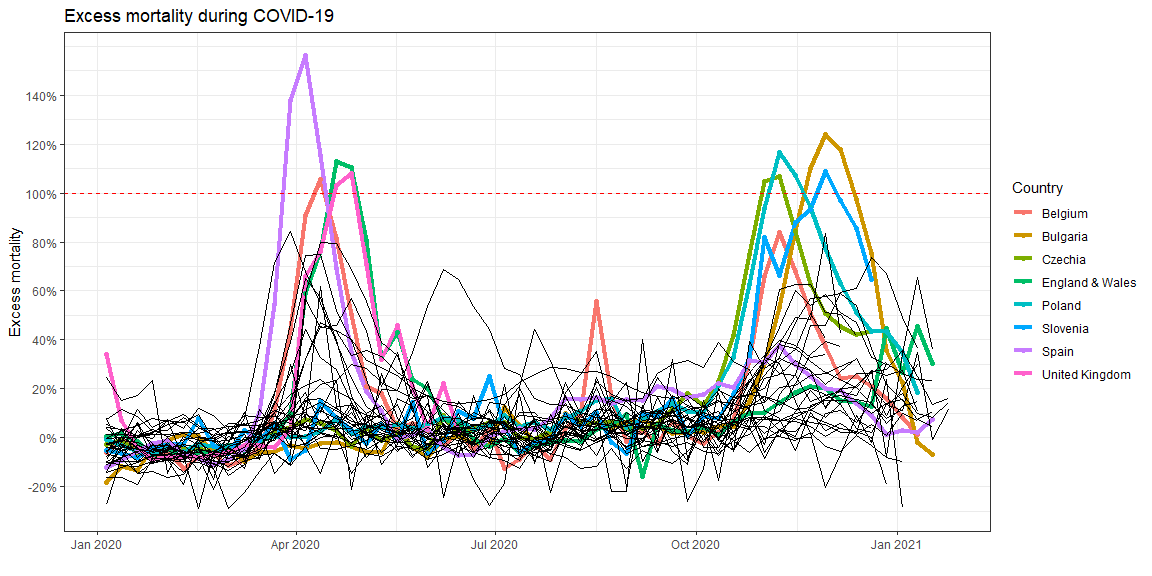
\includegraphics{eda_files/figure-latex/unnamed-chunk-7-1.pdf}
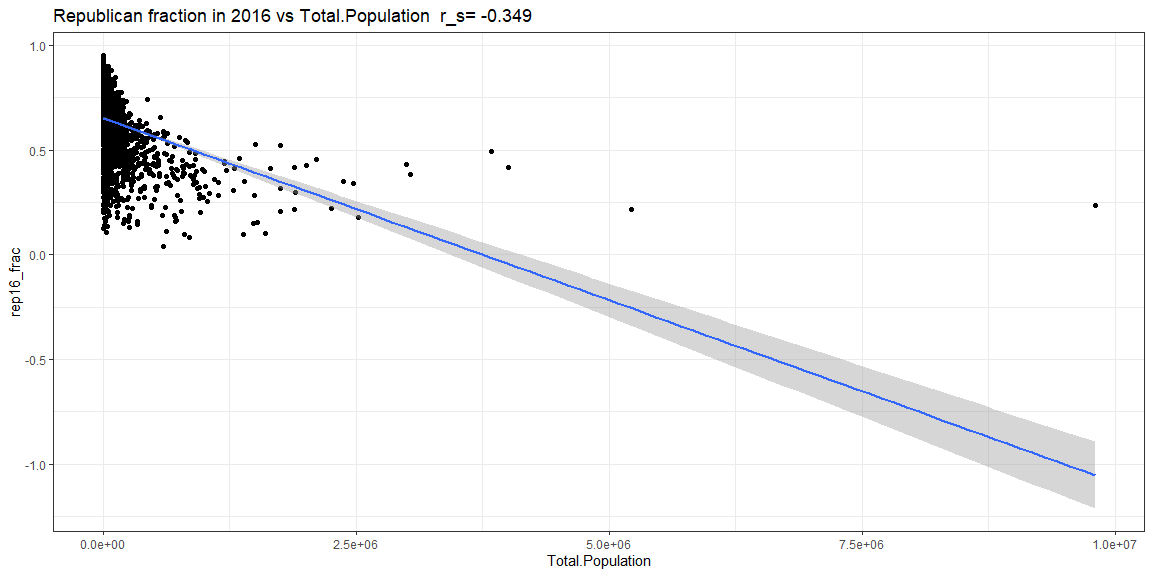
\includegraphics{eda_files/figure-latex/unnamed-chunk-7-2.pdf}
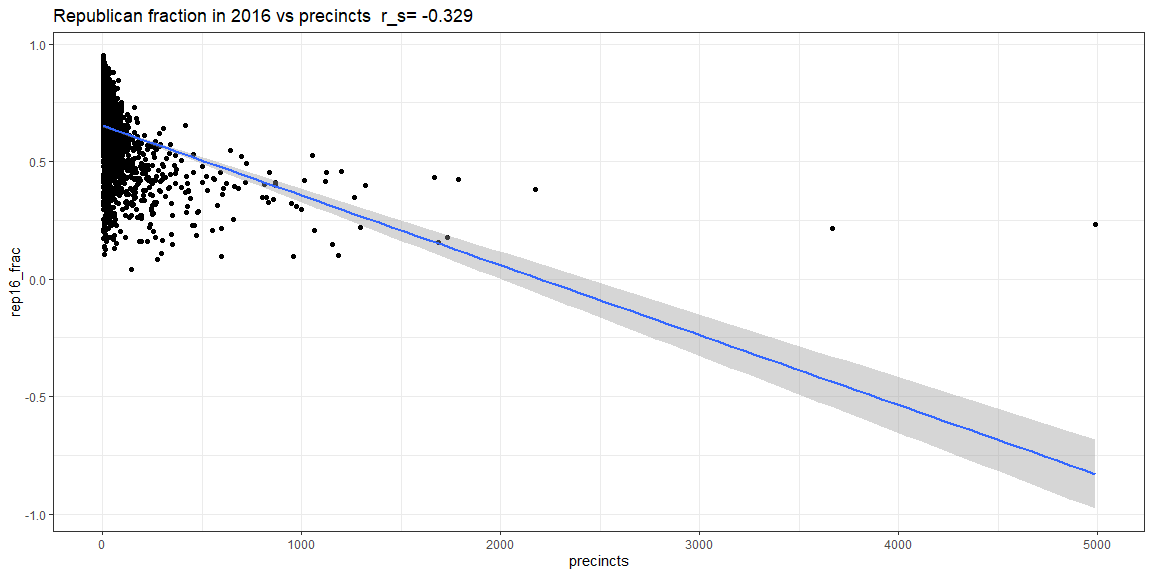
\includegraphics{eda_files/figure-latex/unnamed-chunk-7-3.pdf}
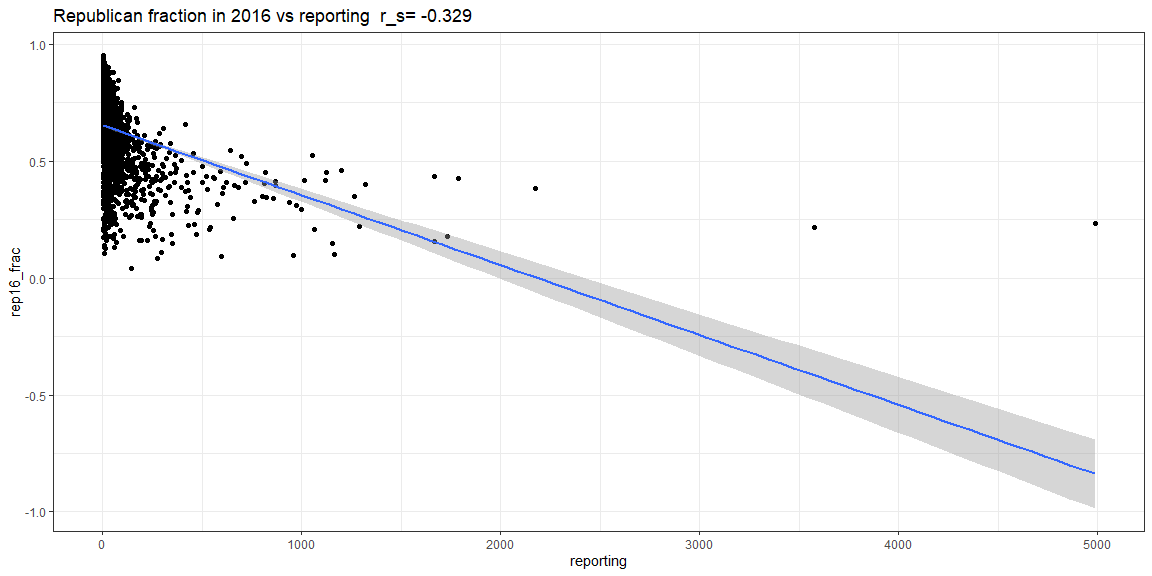
\includegraphics{eda_files/figure-latex/unnamed-chunk-7-4.pdf}
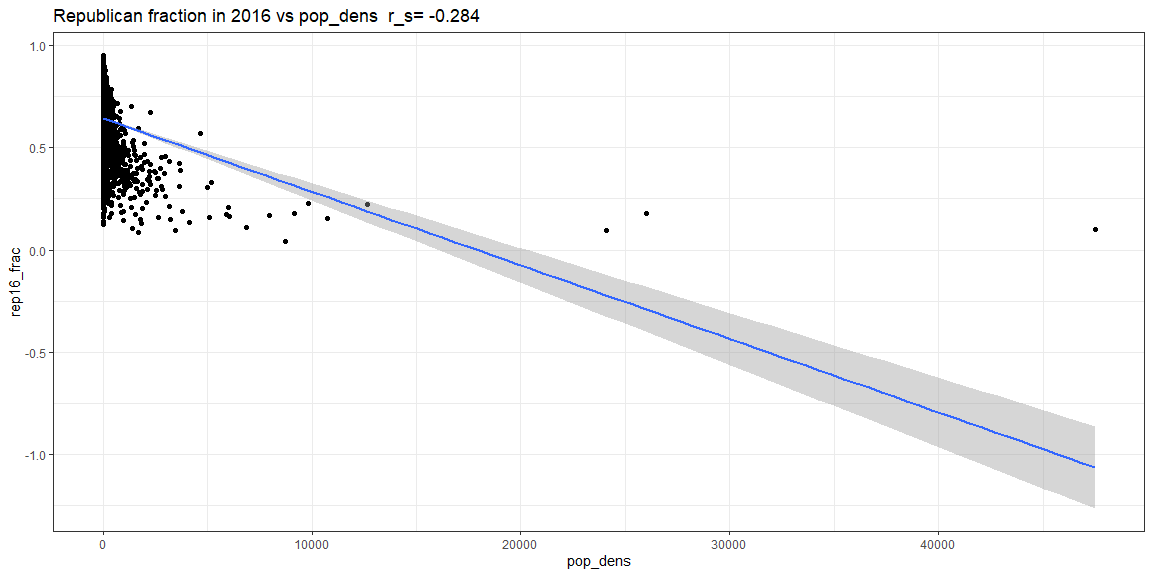
\includegraphics{eda_files/figure-latex/unnamed-chunk-7-5.pdf}
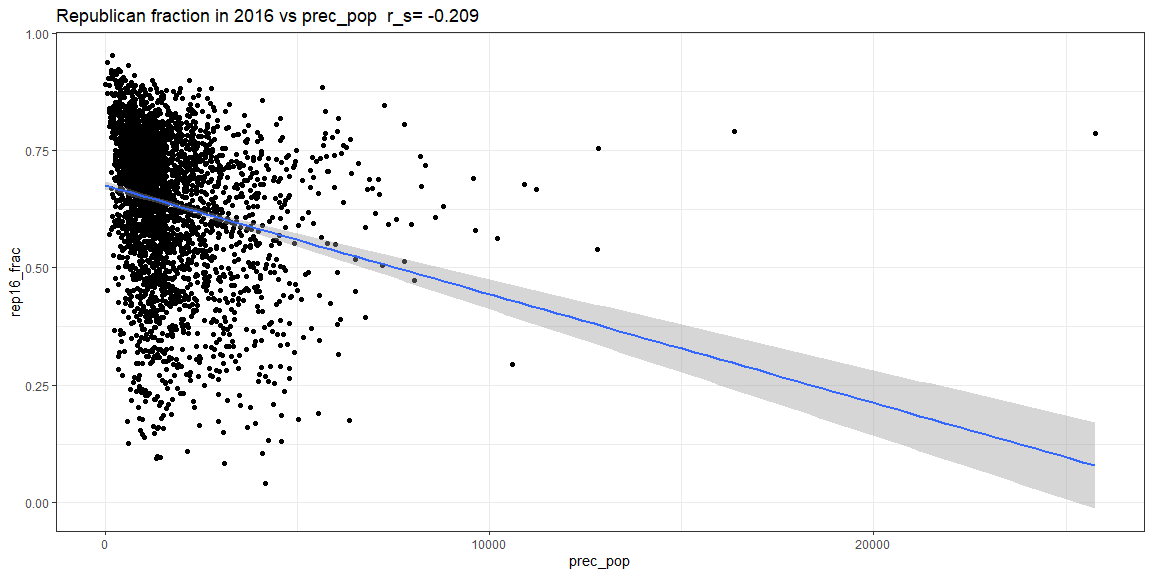
\includegraphics{eda_files/figure-latex/unnamed-chunk-7-6.pdf}
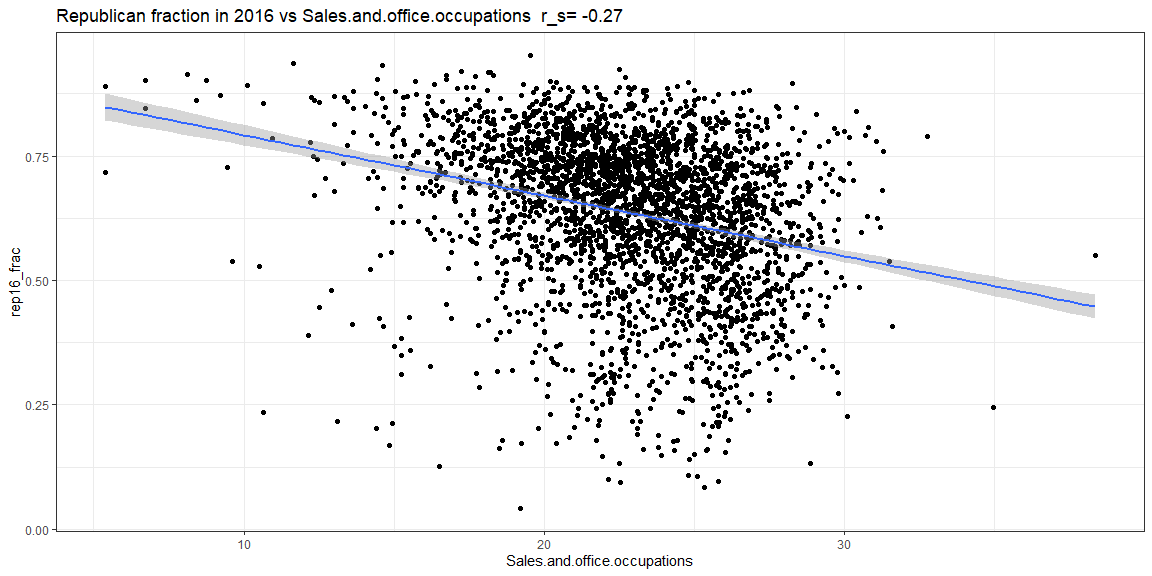
\includegraphics{eda_files/figure-latex/unnamed-chunk-7-7.pdf}
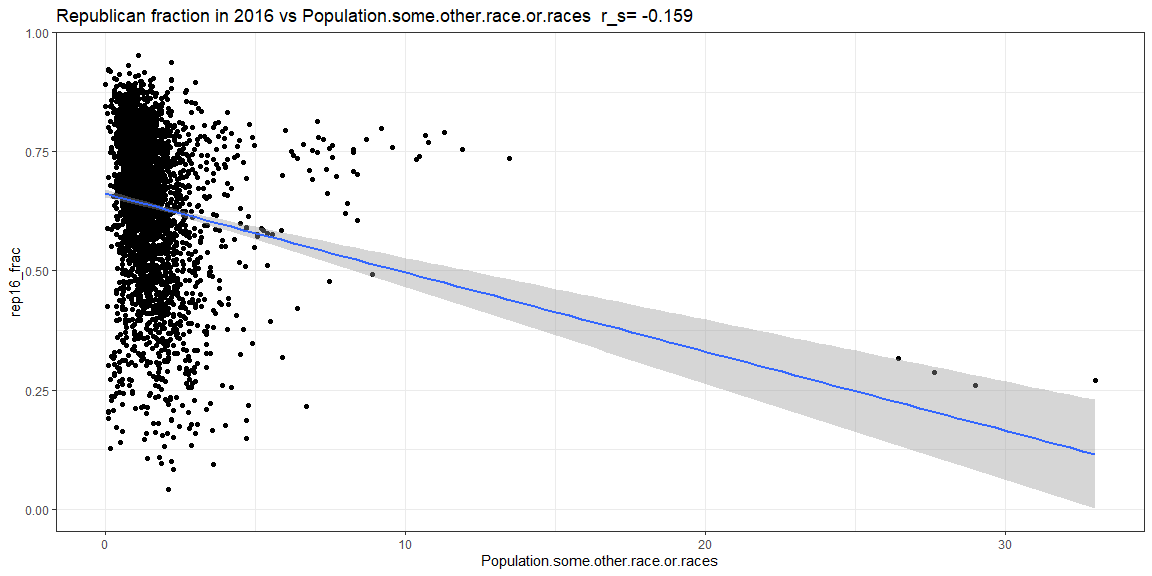
\includegraphics{eda_files/figure-latex/unnamed-chunk-7-8.pdf}

\hypertarget{preparing-the-data-for-prediction}{%
\subsection{Preparing the data for
prediction}\label{preparing-the-data-for-prediction}}

\begin{Shaded}
\begin{Highlighting}[]
\NormalTok{d\_numeric }\OtherTok{\textless{}{-}}\NormalTok{ d[, }\FunctionTok{unlist}\NormalTok{(}\FunctionTok{lapply}\NormalTok{(d, is.numeric))]}
\NormalTok{d\_numeric }\OtherTok{\textless{}{-}}\NormalTok{ d\_numeric }\SpecialCharTok{\%\textgreater{}\%}
  \FunctionTok{rowwise}\NormalTok{() }\SpecialCharTok{\%\textgreater{}\%}
  \FunctionTok{mutate}\NormalTok{(}\AttributeTok{dem16\_win =}\NormalTok{ (rep16\_frac2 }\SpecialCharTok{\textless{}}\NormalTok{ dem16\_frac2)) }\SpecialCharTok{\%\textgreater{}\%}
  \FunctionTok{ungroup}\NormalTok{()}

\NormalTok{d\_cor }\OtherTok{\textless{}{-}}\NormalTok{ d\_numeric }\SpecialCharTok{\%\textgreater{}\%} 
    \FunctionTok{select}\NormalTok{(}\SpecialCharTok{!}\FunctionTok{starts\_with}\NormalTok{(}\StringTok{"vote"}\NormalTok{)) }\SpecialCharTok{\%\textgreater{}\%}
    \FunctionTok{select}\NormalTok{(}\SpecialCharTok{!}\FunctionTok{matches}\NormalTok{(}\StringTok{"...(08|12)\_frac.*"}\NormalTok{)) }\SpecialCharTok{\%\textgreater{}\%}
    \FunctionTok{select}\NormalTok{(}\SpecialCharTok{!}\FunctionTok{matches}\NormalTok{(}\StringTok{"[a{-}z][0{-}9][0{-}9]$"}\NormalTok{)) }\SpecialCharTok{\%\textgreater{}\%}
    \FunctionTok{select}\NormalTok{(}\SpecialCharTok{!}\FunctionTok{ends\_with}\NormalTok{(}\StringTok{"frac2"}\NormalTok{))}
\NormalTok{d\_cor }\OtherTok{\textless{}{-}} 
\NormalTok{  d\_cor[,}\SpecialCharTok{!}\FunctionTok{grepl}\NormalTok{(}\StringTok{"(?\textless{}!rep)16\_frac.*"}\NormalTok{,}\FunctionTok{colnames}\NormalTok{(d\_cor),}\AttributeTok{perl=}\NormalTok{T)]}

\NormalTok{spearman\_cols }\OtherTok{\textless{}{-}} 
  \FunctionTok{row.names}\NormalTok{(}\FunctionTok{as.data.frame}\NormalTok{(}\FunctionTok{cor}\NormalTok{(}
\NormalTok{    d\_cor, }\AttributeTok{use=}\StringTok{"pairwise.complete.obs"}\NormalTok{, }\AttributeTok{method=}\StringTok{"spearman"}
\NormalTok{  )) }\SpecialCharTok{\%\textgreater{}\%}
  \FunctionTok{select}\NormalTok{(rep16\_frac) }\SpecialCharTok{\%\textgreater{}\%}
  \FunctionTok{arrange}\NormalTok{(}\SpecialCharTok{{-}}\FunctionTok{abs}\NormalTok{(rep16\_frac)) }\SpecialCharTok{\%\textgreater{}\%}
  \FunctionTok{head}\NormalTok{(}\DecValTok{15}\NormalTok{) }\SpecialCharTok{\%\textgreater{}\%}
  \FunctionTok{distinct}\NormalTok{(rep16\_frac, }\AttributeTok{.keep\_all =}\NormalTok{ T))}

\NormalTok{pearson\_cols }\OtherTok{\textless{}{-}} 
  \FunctionTok{row.names}\NormalTok{(}\FunctionTok{as.data.frame}\NormalTok{(}\FunctionTok{cor}\NormalTok{(}
\NormalTok{    d\_cor, }\AttributeTok{use=}\StringTok{"pairwise.complete.obs"}\NormalTok{, }\AttributeTok{method=}\StringTok{"pearson"}
\NormalTok{  )) }\SpecialCharTok{\%\textgreater{}\%}
  \FunctionTok{select}\NormalTok{(rep16\_frac) }\SpecialCharTok{\%\textgreater{}\%}
  \FunctionTok{arrange}\NormalTok{(}\SpecialCharTok{{-}}\FunctionTok{abs}\NormalTok{(rep16\_frac)) }\SpecialCharTok{\%\textgreater{}\%}
  \FunctionTok{head}\NormalTok{(}\DecValTok{20}\NormalTok{) }\SpecialCharTok{\%\textgreater{}\%}
  \FunctionTok{distinct}\NormalTok{(rep16\_frac, }\AttributeTok{.keep\_all =}\NormalTok{ T))}

\CommentTok{\# Just these cols give about 91\% testing acc}
\CommentTok{\#pearson\_cols \textless{}{-} c("White","log\_pd","Black","Hispanic")}
\NormalTok{important\_cols }\OtherTok{\textless{}{-}} \FunctionTok{c}\NormalTok{(pearson\_cols, }\StringTok{"dem16\_win"}\NormalTok{,}\StringTok{"fips"}\NormalTok{)}
\CommentTok{\# Sampling will bias towards the less common D counties, }
\CommentTok{\# increasing D recall\&precision but decreasing overall acc }
\NormalTok{d\_dem }\OtherTok{\textless{}{-}}\NormalTok{ d\_numeric }\SpecialCharTok{\%\textgreater{}\%} \FunctionTok{filter}\NormalTok{(dem16\_win) }\CommentTok{\#\%\textgreater{}\% sample\_n(480)}
\NormalTok{d\_rep }\OtherTok{\textless{}{-}}\NormalTok{ d\_numeric }\SpecialCharTok{\%\textgreater{}\%} \FunctionTok{filter}\NormalTok{(}\SpecialCharTok{!}\NormalTok{dem16\_win) }\CommentTok{\#\%\textgreater{}\% sample\_n(480)}
\NormalTok{d\_balanced }\OtherTok{\textless{}{-}} \FunctionTok{bind\_rows}\NormalTok{(d\_dem, d\_rep)}
\NormalTok{d\_ml }\OtherTok{\textless{}{-}}\NormalTok{ d\_balanced }\SpecialCharTok{\%\textgreater{}\%}
  \FunctionTok{select}\NormalTok{(important\_cols) }\SpecialCharTok{\%\textgreater{}\%}
  \FunctionTok{select}\NormalTok{(}\SpecialCharTok{!}\FunctionTok{matches}\NormalTok{(}\StringTok{"\_frac.*"}\NormalTok{)) }\SpecialCharTok{\%\textgreater{}\%}
  \FunctionTok{select}\NormalTok{(}\SpecialCharTok{!}\FunctionTok{starts\_with}\NormalTok{(}\StringTok{"vote"}\NormalTok{)) }\SpecialCharTok{\%\textgreater{}\%}
  \FunctionTok{select}\NormalTok{(}\SpecialCharTok{!}\FunctionTok{matches}\NormalTok{(}\StringTok{"[a{-}z][0{-}9][0{-}9]$"}\NormalTok{))}
\end{Highlighting}
\end{Shaded}

\begin{verbatim}
## Note: Using an external vector in selections is ambiguous.
## i Use `all_of(important_cols)` instead of `important_cols` to silence this message.
## i See <https://tidyselect.r-lib.org/reference/faq-external-vector.html>.
## This message is displayed once per session.
\end{verbatim}

\begin{Shaded}
\begin{Highlighting}[]
\FunctionTok{set.seed}\NormalTok{(seed)}
\NormalTok{d\_train }\OtherTok{\textless{}{-}}\NormalTok{ d\_ml }\SpecialCharTok{\%\textgreater{}\%} \FunctionTok{sample\_frac}\NormalTok{(}\FloatTok{0.8}\NormalTok{)}
\NormalTok{d\_test }\OtherTok{\textless{}{-}} \FunctionTok{anti\_join}\NormalTok{(d\_ml, d\_train, }\AttributeTok{by=}\StringTok{"fips"}\NormalTok{)}
\CommentTok{\# Don\textquotesingle{}t include the fips col}
\NormalTok{d\_train }\OtherTok{\textless{}{-}}\NormalTok{ d\_train }\SpecialCharTok{\%\textgreater{}\%} \FunctionTok{select}\NormalTok{(}\SpecialCharTok{!}\NormalTok{fips)}
\NormalTok{d\_test }\OtherTok{\textless{}{-}}\NormalTok{ d\_test }\SpecialCharTok{\%\textgreater{}\%} \FunctionTok{select}\NormalTok{(}\SpecialCharTok{!}\NormalTok{fips)}
\end{Highlighting}
\end{Shaded}

\hypertarget{decision-tree}{%
\subsection{Decision tree}\label{decision-tree}}

\begin{Shaded}
\begin{Highlighting}[]
\NormalTok{metrics }\OtherTok{\textless{}{-}} \ControlFlowTok{function}\NormalTok{(conf\_matrix, tacc)\{}
\NormalTok{  num\_instances }\OtherTok{\textless{}{-}} \FunctionTok{sum}\NormalTok{(conf\_matrix)}
\NormalTok{  num\_classes }\OtherTok{\textless{}{-}} \FunctionTok{nrow}\NormalTok{(conf\_matrix)}
\NormalTok{  row\_sums }\OtherTok{\textless{}{-}} \FunctionTok{apply}\NormalTok{(conf\_matrix, }\DecValTok{1}\NormalTok{, sum)}
\NormalTok{  col\_sums }\OtherTok{\textless{}{-}} \FunctionTok{apply}\NormalTok{(conf\_matrix, }\DecValTok{2}\NormalTok{, sum)}
\NormalTok{  diags }\OtherTok{\textless{}{-}} \FunctionTok{diag}\NormalTok{(conf\_matrix)}
  
  \CommentTok{\# Calculate evaluation metrics and put in DF}
\NormalTok{  em }\OtherTok{\textless{}{-}} \FunctionTok{data.frame}\NormalTok{(}\AttributeTok{Metric=}\FunctionTok{character}\NormalTok{(),}\AttributeTok{Value=}\FunctionTok{double}\NormalTok{())}
\NormalTok{  em }\OtherTok{\textless{}{-}}\NormalTok{ em }\SpecialCharTok{\%\textgreater{}\%}
    \FunctionTok{add\_row}\NormalTok{(}\AttributeTok{Metric=}\StringTok{"Total acc."}\NormalTok{,}\AttributeTok{Value=}\NormalTok{tacc)}
\NormalTok{  em }\OtherTok{\textless{}{-}}\NormalTok{ em }\SpecialCharTok{\%\textgreater{}\%}
    \FunctionTok{add\_row}\NormalTok{(}\AttributeTok{Metric=}\StringTok{"Accuracy"}\NormalTok{,}\AttributeTok{Value=}\NormalTok{(}\FunctionTok{sum}\NormalTok{(diags) }\SpecialCharTok{/}\NormalTok{ num\_instances))}
\NormalTok{  em }\OtherTok{\textless{}{-}}\NormalTok{ em }\SpecialCharTok{\%\textgreater{}\%}
    \FunctionTok{add\_row}\NormalTok{(}\AttributeTok{Metric=}\StringTok{"Precision"}\NormalTok{,}\AttributeTok{Value=}\NormalTok{(diags }\SpecialCharTok{/}\NormalTok{ col\_sums))}
\NormalTok{  em }\OtherTok{\textless{}{-}}\NormalTok{ em }\SpecialCharTok{\%\textgreater{}\%}
    \FunctionTok{add\_row}\NormalTok{(}\AttributeTok{Metric=}\StringTok{"Recall"}\NormalTok{,}\AttributeTok{Value=}\NormalTok{(diags }\SpecialCharTok{/}\NormalTok{ row\_sums))}
  \FunctionTok{return}\NormalTok{(em)}
\NormalTok{\}}
\end{Highlighting}
\end{Shaded}

\begin{Shaded}
\begin{Highlighting}[]
\NormalTok{my\_tree }\OtherTok{\textless{}{-}} \FunctionTok{rpart}\NormalTok{(}
  \FunctionTok{as.factor}\NormalTok{(dem16\_win) }\SpecialCharTok{\textasciitilde{}}\NormalTok{ ., }\AttributeTok{data=}\NormalTok{d\_train, }\AttributeTok{method=}\StringTok{"class"}\NormalTok{,}
  \AttributeTok{control=}\FunctionTok{rpart.control}\NormalTok{(}\AttributeTok{maxdepth=}\DecValTok{10}\NormalTok{,}\AttributeTok{xval=}\DecValTok{30}\NormalTok{))}
\CommentTok{\# 0.01{-}0.025 seems to be the best complexity parameter value}
\CommentTok{\# Now 0.013{-}0.017 seems to be about the best}
\CommentTok{\# 0.11 seems close to optimal, but pruning doesn\textquotesingle{}t seem to help}
\CommentTok{\# much}
\NormalTok{my\_tree }\OtherTok{\textless{}{-}} \FunctionTok{prune}\NormalTok{(my\_tree,}\AttributeTok{cp=}\FloatTok{0.011}\NormalTok{)}
\NormalTok{d\_tst\_pred }\OtherTok{\textless{}{-}} \FunctionTok{predict}\NormalTok{(my\_tree, d\_test, }\AttributeTok{type=}\StringTok{"class"}\NormalTok{)}
\end{Highlighting}
\end{Shaded}

\hypertarget{evalulation-metrics}{%
\subsubsection{Evalulation Metrics}\label{evalulation-metrics}}

\begin{Shaded}
\begin{Highlighting}[]
\CommentTok{\# Calculate evaluation metrics}
\NormalTok{conf\_matrix }\OtherTok{\textless{}{-}} 
  \FunctionTok{as.matrix}\NormalTok{(}\FunctionTok{table}\NormalTok{(}\AttributeTok{predicted =}\NormalTok{ d\_tst\_pred, }\AttributeTok{actual =}\NormalTok{ d\_test}\SpecialCharTok{$}\NormalTok{dem16\_win))}
\NormalTok{d\_pred }\OtherTok{\textless{}{-}} \FunctionTok{predict}\NormalTok{(my\_tree, d\_ml, }\AttributeTok{type=}\StringTok{"class"}\NormalTok{)}
\NormalTok{d\_matrix }\OtherTok{\textless{}{-}} 
  \FunctionTok{as.matrix}\NormalTok{(}\FunctionTok{table}\NormalTok{(}\AttributeTok{predicted =}\NormalTok{ d\_pred, }\AttributeTok{actual =}\NormalTok{ d\_ml}\SpecialCharTok{$}\NormalTok{dem16\_win))}
\NormalTok{tacc }\OtherTok{\textless{}{-}}\NormalTok{ (}\FunctionTok{sum}\NormalTok{(}\FunctionTok{diag}\NormalTok{(d\_matrix)) }\SpecialCharTok{/} \FunctionTok{sum}\NormalTok{(d\_matrix))}
\NormalTok{em }\OtherTok{\textless{}{-}} \FunctionTok{metrics}\NormalTok{(conf\_matrix,tacc)}

\CommentTok{\# Print results}
\NormalTok{knitr}\SpecialCharTok{::}\FunctionTok{kable}\NormalTok{(em)}
\end{Highlighting}
\end{Shaded}

\begin{longtable}[]{@{}lr@{}}
\toprule
Metric & Value \\
\midrule
\endhead
Total acc. & 0.9440514 \\
Accuracy & 0.9292605 \\
Precision & 0.9734345 \\
Precision & 0.6842105 \\
Recall & 0.9447514 \\
Recall & 0.8227848 \\
\bottomrule
\end{longtable}

\begin{Shaded}
\begin{Highlighting}[]
\NormalTok{knitr}\SpecialCharTok{::}\FunctionTok{kable}\NormalTok{(conf\_matrix)}
\end{Highlighting}
\end{Shaded}

\begin{longtable}[]{@{}lrr@{}}
\toprule
& FALSE & TRUE \\
\midrule
\endhead
FALSE & 513 & 30 \\
TRUE & 14 & 65 \\
\bottomrule
\end{longtable}

\begin{Shaded}
\begin{Highlighting}[]
\NormalTok{d\_trn\_pred }\OtherTok{\textless{}{-}} \FunctionTok{predict}\NormalTok{(my\_tree, d\_train, }\AttributeTok{type=}\StringTok{"class"}\NormalTok{)}
\CommentTok{\#knitr::kable(table(predicted = d\_trn\_pred, actual = d\_train$dem16\_win))}
\NormalTok{knitr}\SpecialCharTok{::}\FunctionTok{kable}\NormalTok{(d\_matrix)}
\end{Highlighting}
\end{Shaded}

\begin{longtable}[]{@{}lrr@{}}
\toprule
& FALSE & TRUE \\
\midrule
\endhead
FALSE & 2575 & 124 \\
TRUE & 50 & 361 \\
\bottomrule
\end{longtable}

In the decision tree, it is better NOT to balance the dataset (equal
number of R and D counties) because then it will be biased towards the
less common D counties.

\begin{Shaded}
\begin{Highlighting}[]
\FunctionTok{fancyRpartPlot}\NormalTok{(my\_tree)}
\end{Highlighting}
\end{Shaded}

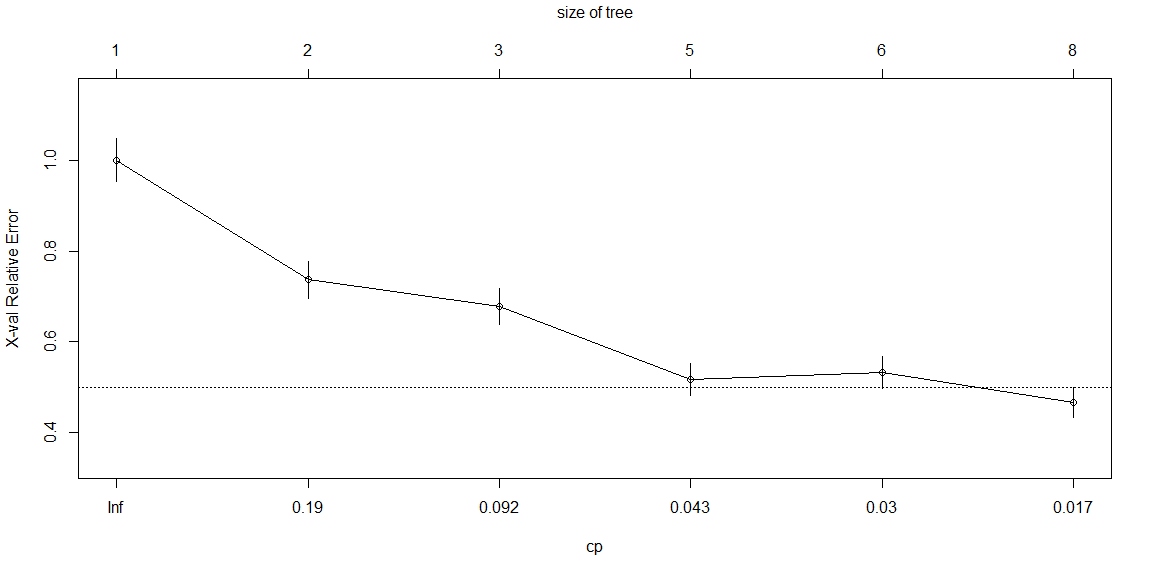
\includegraphics{eda_files/figure-latex/unnamed-chunk-12-1.pdf}

\begin{Shaded}
\begin{Highlighting}[]
\CommentTok{\#printcp(my\_tree)}
\FunctionTok{plotcp}\NormalTok{(my\_tree)}
\end{Highlighting}
\end{Shaded}

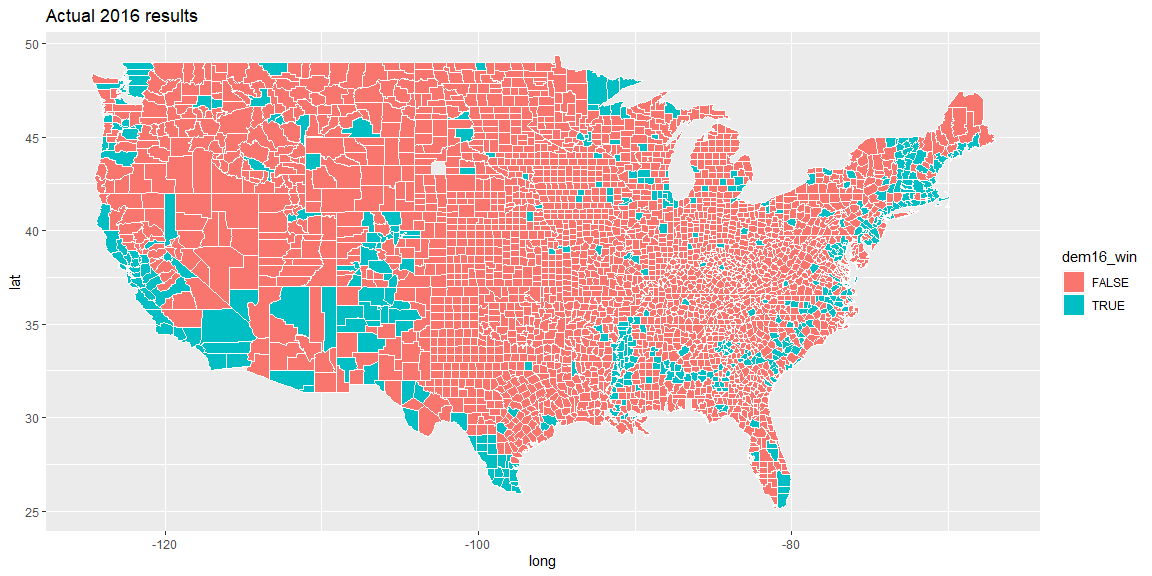
\includegraphics{eda_files/figure-latex/unnamed-chunk-13-1.pdf}

\begin{Shaded}
\begin{Highlighting}[]
\CommentTok{\#my\_tree \textless{}{-} prune(my\_tree,cp=0.017)}
\FunctionTok{fancyRpartPlot}\NormalTok{(my\_tree)}
\end{Highlighting}
\end{Shaded}

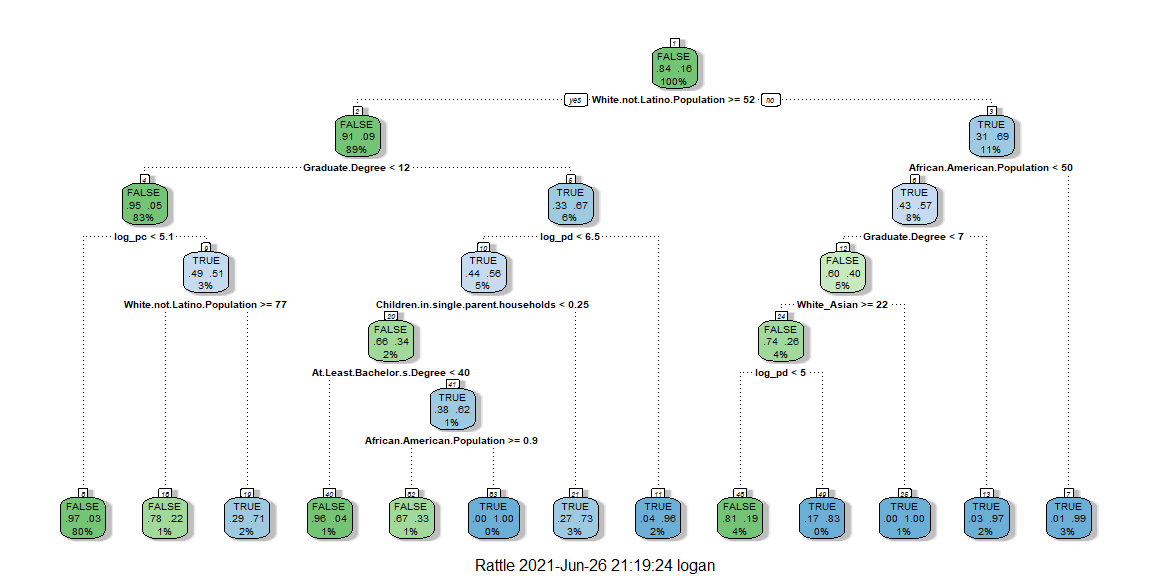
\includegraphics{eda_files/figure-latex/unnamed-chunk-13-2.pdf}

\hypertarget{graphing-results}{%
\subsubsection{Graphing Results}\label{graphing-results}}

\begin{Shaded}
\begin{Highlighting}[]
\NormalTok{d\_wins }\OtherTok{\textless{}{-}}\NormalTok{ d }\SpecialCharTok{\%\textgreater{}\%}
  \FunctionTok{rowwise}\NormalTok{() }\SpecialCharTok{\%\textgreater{}\%}
  \FunctionTok{mutate}\NormalTok{(}\AttributeTok{dem16\_win =}\NormalTok{ (rep16\_frac2 }\SpecialCharTok{\textless{}}\NormalTok{ dem16\_frac2)) }\SpecialCharTok{\%\textgreater{}\%}
  \FunctionTok{ungroup}\NormalTok{()}
\NormalTok{d\_preds }\OtherTok{\textless{}{-}}\NormalTok{ d\_wins }\SpecialCharTok{\%\textgreater{}\%}
  \FunctionTok{select}\NormalTok{(fips, dem16\_win)}
\NormalTok{predictions }\OtherTok{\textless{}{-}} 
  \FunctionTok{as.data.frame}\NormalTok{(}\FunctionTok{predict}\NormalTok{(my\_tree, d\_wins, }\AttributeTok{type=}\StringTok{"class"}\NormalTok{)) }\SpecialCharTok{\%\textgreater{}\%}
  \FunctionTok{pull}\NormalTok{()}
\NormalTok{d\_preds}\SpecialCharTok{$}\NormalTok{pred\_win }\OtherTok{=}\NormalTok{ predictions}
\NormalTok{c\_fips }\OtherTok{\textless{}{-}}\NormalTok{ county.fips }\SpecialCharTok{\%\textgreater{}\%}
  \FunctionTok{separate}\NormalTok{(polyname, }\FunctionTok{c}\NormalTok{(}\StringTok{"region"}\NormalTok{,}\StringTok{"subregion"}\NormalTok{), }\AttributeTok{sep=}\StringTok{","}\NormalTok{)}
\NormalTok{cty\_shape\_fips }\OtherTok{\textless{}{-}}
  \FunctionTok{inner\_join}\NormalTok{(}\FunctionTok{map\_data}\NormalTok{(}\StringTok{"county"}\NormalTok{),c\_fips,}\AttributeTok{by=}\FunctionTok{c}\NormalTok{(}\StringTok{"region"}\NormalTok{,}\StringTok{"subregion"}\NormalTok{))}
\NormalTok{d\_graph }\OtherTok{\textless{}{-}} \FunctionTok{inner\_join}\NormalTok{(d\_preds,cty\_shape\_fips,}\AttributeTok{by=}\StringTok{"fips"}\NormalTok{)}
\end{Highlighting}
\end{Shaded}

\begin{Shaded}
\begin{Highlighting}[]
\FunctionTok{ggplot}\NormalTok{(d\_graph) }\SpecialCharTok{+}
    \FunctionTok{geom\_polygon}\NormalTok{(}\FunctionTok{aes}\NormalTok{(}\AttributeTok{x=}\NormalTok{long,}\AttributeTok{y=}\NormalTok{lat,}\AttributeTok{group=}\NormalTok{group,}\AttributeTok{fill=}\NormalTok{dem16\_win),}
                 \AttributeTok{color=}\StringTok{"white"}\NormalTok{) }\SpecialCharTok{+}
    \FunctionTok{ggtitle}\NormalTok{(}\StringTok{"Actual 2016 results"}\NormalTok{)}
\end{Highlighting}
\end{Shaded}

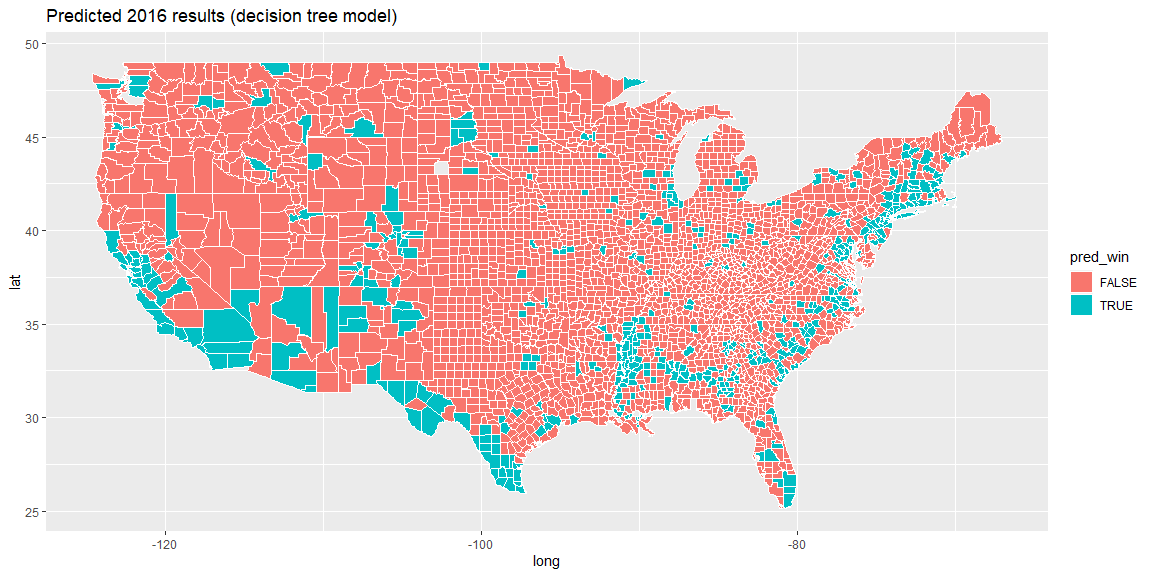
\includegraphics{eda_files/figure-latex/unnamed-chunk-15-1.pdf}

\begin{Shaded}
\begin{Highlighting}[]
\FunctionTok{ggplot}\NormalTok{(d\_graph) }\SpecialCharTok{+}
    \FunctionTok{geom\_polygon}\NormalTok{(}\FunctionTok{aes}\NormalTok{(}\AttributeTok{x=}\NormalTok{long,}\AttributeTok{y=}\NormalTok{lat,}\AttributeTok{group=}\NormalTok{group,}\AttributeTok{fill=}\NormalTok{pred\_win),}
                 \AttributeTok{color=}\StringTok{"white"}\NormalTok{) }\SpecialCharTok{+}
    \FunctionTok{ggtitle}\NormalTok{(}\StringTok{"Predicted 2016 results (decision tree model)"}\NormalTok{)}
\end{Highlighting}
\end{Shaded}

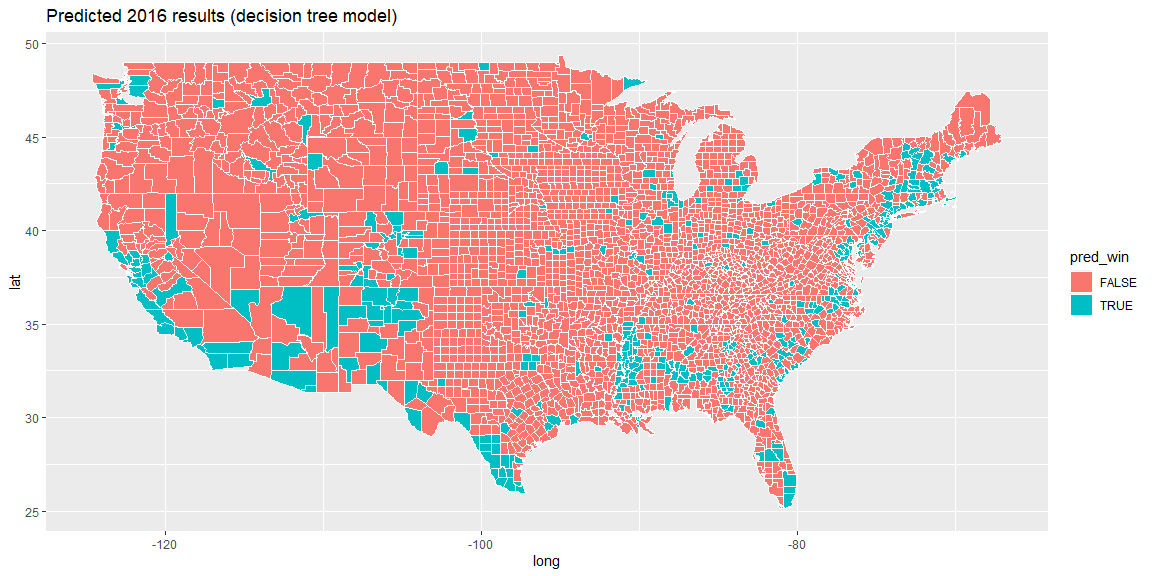
\includegraphics{eda_files/figure-latex/unnamed-chunk-16-1.pdf}

\hypertarget{linear-regression}{%
\subsection{Linear regression}\label{linear-regression}}

\begin{Shaded}
\begin{Highlighting}[]
\CommentTok{\# Create the model}
\FunctionTok{set.seed}\NormalTok{(seed)}
\NormalTok{d\_ml2 }\OtherTok{\textless{}{-}}\NormalTok{ d\_numeric }\SpecialCharTok{\%\textgreater{}\%}
    \FunctionTok{mutate}\NormalTok{(}\AttributeTok{dem16\_win =}\NormalTok{ (rep16\_frac2 }\SpecialCharTok{\textless{}}\NormalTok{ dem16\_frac2))}
\NormalTok{d\_train\_l }\OtherTok{\textless{}{-}}\NormalTok{ d\_ml2 }\SpecialCharTok{\%\textgreater{}\%} \FunctionTok{sample\_frac}\NormalTok{(}\FloatTok{0.8}\NormalTok{)}
\NormalTok{d\_test\_l }\OtherTok{\textless{}{-}} \FunctionTok{anti\_join}\NormalTok{(d\_ml2, d\_train\_l, }\AttributeTok{by=}\StringTok{"fips"}\NormalTok{)}
\CommentTok{\# Teen birth data seems hard to come by}
\NormalTok{mylm }\OtherTok{\textless{}{-}}
  \FunctionTok{lm}\NormalTok{(dem16\_frac2 }\SpecialCharTok{\textasciitilde{}}\NormalTok{ White }\SpecialCharTok{+}\NormalTok{ Black }\SpecialCharTok{+}\NormalTok{ Graduate.Degree }\SpecialCharTok{+}\NormalTok{ log\_pd }\SpecialCharTok{+}\NormalTok{ lat }\SpecialCharTok{+}\NormalTok{ White}\SpecialCharTok{:}\NormalTok{lat }\SpecialCharTok{+}\NormalTok{ median\_age }\SpecialCharTok{+}\NormalTok{ White}\SpecialCharTok{:}\NormalTok{Black }\SpecialCharTok{+}\NormalTok{ White}\SpecialCharTok{:}\NormalTok{Hispanic }\SpecialCharTok{+}\NormalTok{ White}\SpecialCharTok{:}\NormalTok{Graduate.Degree }\SpecialCharTok{+}\NormalTok{ White}\SpecialCharTok{:}\NormalTok{lon, }\AttributeTok{data=}\NormalTok{d\_train\_l)}

\CommentTok{\# Predict}
\NormalTok{thresh }\OtherTok{\textless{}{-}} \FloatTok{0.5}
\NormalTok{d\_tst\_pred\_l }\OtherTok{\textless{}{-}}\NormalTok{ (}\FunctionTok{predict}\NormalTok{(mylm, d\_test\_l) }\SpecialCharTok{\textgreater{}}\NormalTok{ thresh)}
\NormalTok{conf\_matrix\_l }\OtherTok{\textless{}{-}} 
  \FunctionTok{as.matrix}\NormalTok{(}\FunctionTok{table}\NormalTok{(}\AttributeTok{predicted =}\NormalTok{ d\_tst\_pred\_l, }\AttributeTok{actual =}\NormalTok{ d\_test\_l}\SpecialCharTok{$}\NormalTok{dem16\_win))}
\NormalTok{d\_pred\_l }\OtherTok{\textless{}{-}}\NormalTok{ (}\FunctionTok{predict}\NormalTok{(mylm, d\_ml2) }\SpecialCharTok{\textgreater{}}\NormalTok{ thresh)}
\NormalTok{d\_matrix\_l }\OtherTok{\textless{}{-}} 
  \FunctionTok{as.matrix}\NormalTok{(}\FunctionTok{table}\NormalTok{(}\AttributeTok{predicted =}\NormalTok{ d\_pred\_l, }\AttributeTok{actual =}\NormalTok{ d\_ml2}\SpecialCharTok{$}\NormalTok{dem16\_win))}
\NormalTok{tacc\_l }\OtherTok{\textless{}{-}}\NormalTok{ (}\FunctionTok{sum}\NormalTok{(}\FunctionTok{diag}\NormalTok{(d\_matrix\_l)) }\SpecialCharTok{/} \FunctionTok{sum}\NormalTok{(d\_matrix\_l))}

\CommentTok{\# Get evaluation metrics}
\NormalTok{em }\OtherTok{\textless{}{-}} \FunctionTok{metrics}\NormalTok{(conf\_matrix\_l,tacc\_l)}

\CommentTok{\# Show metrics}
\NormalTok{knitr}\SpecialCharTok{::}\FunctionTok{kable}\NormalTok{(em)}
\end{Highlighting}
\end{Shaded}

\begin{longtable}[]{@{}lr@{}}
\toprule
Metric & Value \\
\midrule
\endhead
Total acc. & 0.9395498 \\
Accuracy & 0.9466882 \\
Precision & 0.9868914 \\
Precision & 0.6941176 \\
Recall & 0.9529837 \\
Recall & 0.8939394 \\
\bottomrule
\end{longtable}

\begin{Shaded}
\begin{Highlighting}[]
\NormalTok{knitr}\SpecialCharTok{::}\FunctionTok{kable}\NormalTok{(conf\_matrix\_l)}
\end{Highlighting}
\end{Shaded}

\begin{longtable}[]{@{}lrr@{}}
\toprule
& FALSE & TRUE \\
\midrule
\endhead
FALSE & 527 & 26 \\
TRUE & 7 & 59 \\
\bottomrule
\end{longtable}

\begin{Shaded}
\begin{Highlighting}[]
\NormalTok{knitr}\SpecialCharTok{::}\FunctionTok{kable}\NormalTok{(d\_matrix\_l)}
\end{Highlighting}
\end{Shaded}

\begin{longtable}[]{@{}lrr@{}}
\toprule
& FALSE & TRUE \\
\midrule
\endhead
FALSE & 2574 & 137 \\
TRUE & 51 & 348 \\
\bottomrule
\end{longtable}

\hypertarget{graphing-results-1}{%
\subsubsection{Graphing results}\label{graphing-results-1}}

\begin{Shaded}
\begin{Highlighting}[]
\NormalTok{d\_wins }\OtherTok{\textless{}{-}}\NormalTok{ d }\SpecialCharTok{\%\textgreater{}\%}
  \FunctionTok{rowwise}\NormalTok{() }\SpecialCharTok{\%\textgreater{}\%}
  \FunctionTok{mutate}\NormalTok{(}\AttributeTok{dem16\_win =}\NormalTok{ (rep16\_frac2 }\SpecialCharTok{\textless{}}\NormalTok{ dem16\_frac2)) }\SpecialCharTok{\%\textgreater{}\%}
  \FunctionTok{ungroup}\NormalTok{()}
\NormalTok{d\_preds\_l }\OtherTok{\textless{}{-}}\NormalTok{ d\_wins }\SpecialCharTok{\%\textgreater{}\%}
  \FunctionTok{select}\NormalTok{(fips, dem16\_win)}
\NormalTok{predictions }\OtherTok{\textless{}{-}} 
  \FunctionTok{as.data.frame}\NormalTok{((}\FunctionTok{predict}\NormalTok{(mylm, d\_wins) }\SpecialCharTok{\textgreater{}}\NormalTok{ thresh)) }\SpecialCharTok{\%\textgreater{}\%}
  \FunctionTok{pull}\NormalTok{()}
\NormalTok{d\_preds}\SpecialCharTok{$}\NormalTok{pred\_win }\OtherTok{=}\NormalTok{ predictions}
\NormalTok{c\_fips }\OtherTok{\textless{}{-}}\NormalTok{ county.fips }\SpecialCharTok{\%\textgreater{}\%}
  \FunctionTok{separate}\NormalTok{(polyname, }\FunctionTok{c}\NormalTok{(}\StringTok{"region"}\NormalTok{,}\StringTok{"subregion"}\NormalTok{), }\AttributeTok{sep=}\StringTok{","}\NormalTok{)}
\NormalTok{cty\_shape\_fips }\OtherTok{\textless{}{-}}
  \FunctionTok{inner\_join}\NormalTok{(}\FunctionTok{map\_data}\NormalTok{(}\StringTok{"county"}\NormalTok{),c\_fips,}\AttributeTok{by=}\FunctionTok{c}\NormalTok{(}\StringTok{"region"}\NormalTok{,}\StringTok{"subregion"}\NormalTok{))}
\NormalTok{d\_graph\_l }\OtherTok{\textless{}{-}} \FunctionTok{inner\_join}\NormalTok{(d\_preds,cty\_shape\_fips,}\AttributeTok{by=}\StringTok{"fips"}\NormalTok{)}
\end{Highlighting}
\end{Shaded}

\begin{Shaded}
\begin{Highlighting}[]
\FunctionTok{ggplot}\NormalTok{(d\_graph\_l) }\SpecialCharTok{+}
    \FunctionTok{geom\_polygon}\NormalTok{(}\FunctionTok{aes}\NormalTok{(}\AttributeTok{x=}\NormalTok{long,}\AttributeTok{y=}\NormalTok{lat,}\AttributeTok{group=}\NormalTok{group,}\AttributeTok{fill=}\NormalTok{dem16\_win),}
                 \AttributeTok{color=}\StringTok{"white"}\NormalTok{) }\SpecialCharTok{+}
    \FunctionTok{ggtitle}\NormalTok{(}\StringTok{"Actual 2016 results"}\NormalTok{)}
\end{Highlighting}
\end{Shaded}

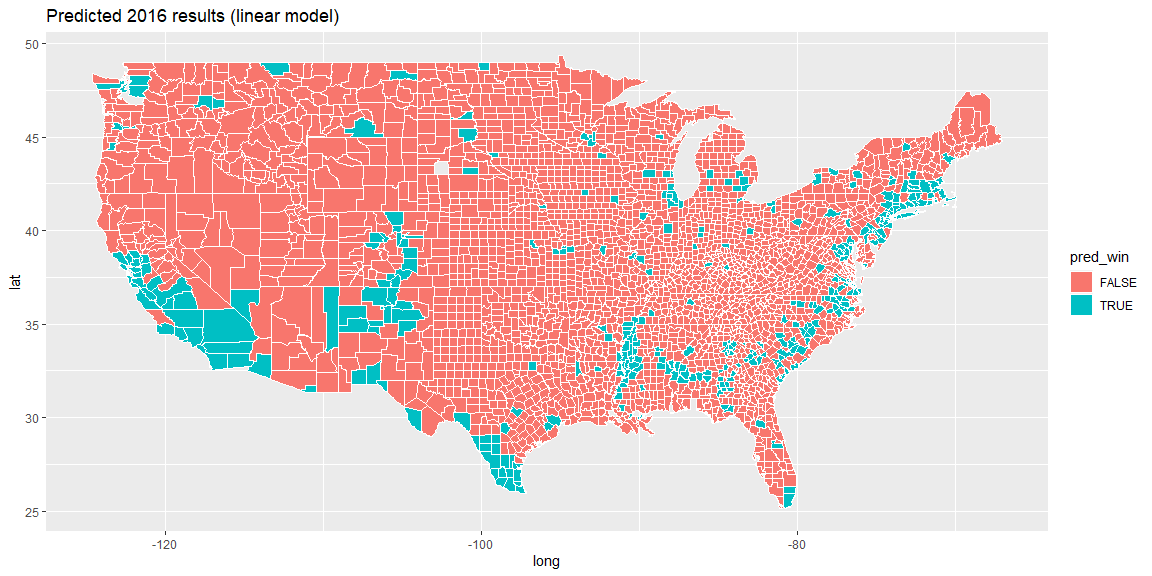
\includegraphics{eda_files/figure-latex/unnamed-chunk-19-1.pdf}

\begin{Shaded}
\begin{Highlighting}[]
\FunctionTok{ggplot}\NormalTok{(d\_graph\_l) }\SpecialCharTok{+}
    \FunctionTok{geom\_polygon}\NormalTok{(}\FunctionTok{aes}\NormalTok{(}\AttributeTok{x=}\NormalTok{long,}\AttributeTok{y=}\NormalTok{lat,}\AttributeTok{group=}\NormalTok{group,}\AttributeTok{fill=}\NormalTok{pred\_win),}
                 \AttributeTok{color=}\StringTok{"white"}\NormalTok{) }\SpecialCharTok{+}
    \FunctionTok{ggtitle}\NormalTok{(}\StringTok{"Predicted 2016 results (linear model)"}\NormalTok{)}
\end{Highlighting}
\end{Shaded}

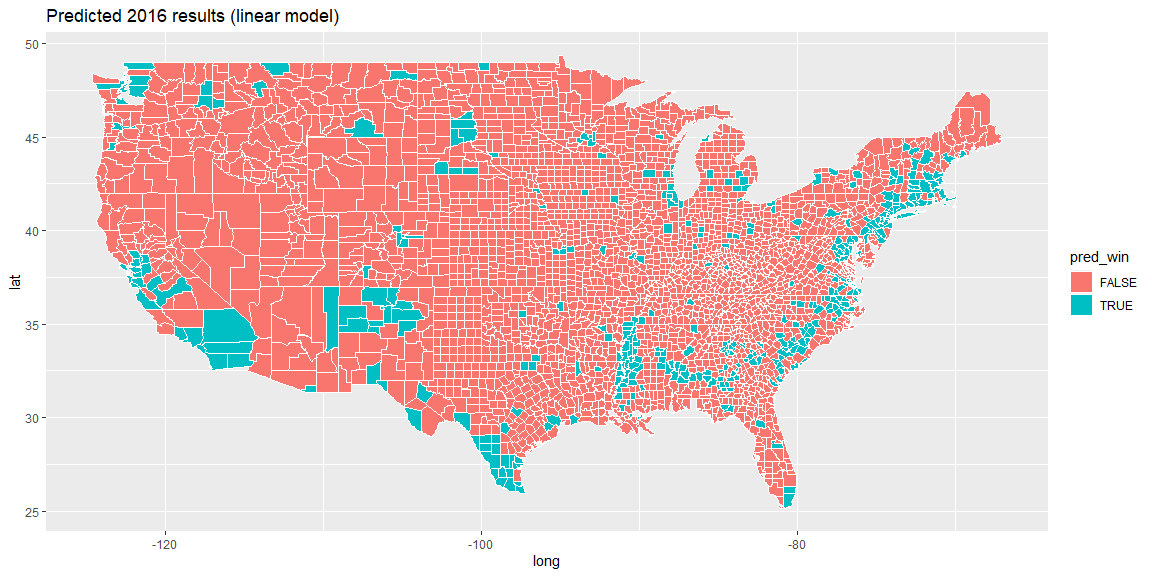
\includegraphics{eda_files/figure-latex/unnamed-chunk-20-1.pdf}

\end{document}
